% Options for packages loaded elsewhere
\PassOptionsToPackage{unicode}{hyperref}
\PassOptionsToPackage{hyphens}{url}
%
\documentclass[
]{article}
\usepackage{amsmath,amssymb}
\usepackage{lmodern}
\usepackage{iftex}
\ifPDFTeX
  \usepackage[T1]{fontenc}
  \usepackage[utf8]{inputenc}
  \usepackage{textcomp} % provide euro and other symbols
\else % if luatex or xetex
  \usepackage{unicode-math}
  \defaultfontfeatures{Scale=MatchLowercase}
  \defaultfontfeatures[\rmfamily]{Ligatures=TeX,Scale=1}
\fi
% Use upquote if available, for straight quotes in verbatim environments
\IfFileExists{upquote.sty}{\usepackage{upquote}}{}
\IfFileExists{microtype.sty}{% use microtype if available
  \usepackage[]{microtype}
  \UseMicrotypeSet[protrusion]{basicmath} % disable protrusion for tt fonts
}{}
\makeatletter
\@ifundefined{KOMAClassName}{% if non-KOMA class
  \IfFileExists{parskip.sty}{%
    \usepackage{parskip}
  }{% else
    \setlength{\parindent}{0pt}
    \setlength{\parskip}{6pt plus 2pt minus 1pt}}
}{% if KOMA class
  \KOMAoptions{parskip=half}}
\makeatother
\usepackage{xcolor}
\usepackage[margin=1in]{geometry}
\usepackage{longtable,booktabs,array}
\usepackage{calc} % for calculating minipage widths
% Correct order of tables after \paragraph or \subparagraph
\usepackage{etoolbox}
\makeatletter
\patchcmd\longtable{\par}{\if@noskipsec\mbox{}\fi\par}{}{}
\makeatother
% Allow footnotes in longtable head/foot
\IfFileExists{footnotehyper.sty}{\usepackage{footnotehyper}}{\usepackage{footnote}}
\makesavenoteenv{longtable}
\usepackage{graphicx}
\makeatletter
\def\maxwidth{\ifdim\Gin@nat@width>\linewidth\linewidth\else\Gin@nat@width\fi}
\def\maxheight{\ifdim\Gin@nat@height>\textheight\textheight\else\Gin@nat@height\fi}
\makeatother
% Scale images if necessary, so that they will not overflow the page
% margins by default, and it is still possible to overwrite the defaults
% using explicit options in \includegraphics[width, height, ...]{}
\setkeys{Gin}{width=\maxwidth,height=\maxheight,keepaspectratio}
% Set default figure placement to htbp
\makeatletter
\def\fps@figure{htbp}
\makeatother
\setlength{\emergencystretch}{3em} % prevent overfull lines
\providecommand{\tightlist}{%
  \setlength{\itemsep}{0pt}\setlength{\parskip}{0pt}}
\setcounter{secnumdepth}{-\maxdimen} % remove section numbering
\usepackage{xcolor}
\definecolor{aliceblue}{HTML}{F0F8FF}
\definecolor{antiquewhite}{HTML}{FAEBD7}
\definecolor{aqua}{HTML}{00FFFF}
\definecolor{aquamarine}{HTML}{7FFFD4}
\definecolor{azure}{HTML}{F0FFFF}
\definecolor{beige}{HTML}{F5F5DC}
\definecolor{bisque}{HTML}{FFE4C4}
\definecolor{black}{HTML}{000000}
\definecolor{blanchedalmond}{HTML}{FFEBCD}
\definecolor{blue}{HTML}{0000FF}
\definecolor{blueviolet}{HTML}{8A2BE2}
\definecolor{brown}{HTML}{A52A2A}
\definecolor{burlywood}{HTML}{DEB887}
\definecolor{cadetblue}{HTML}{5F9EA0}
\definecolor{chartreuse}{HTML}{7FFF00}
\definecolor{chocolate}{HTML}{D2691E}
\definecolor{coral}{HTML}{FF7F50}
\definecolor{cornflowerblue}{HTML}{6495ED}
\definecolor{cornsilk}{HTML}{FFF8DC}
\definecolor{crimson}{HTML}{DC143C}
\definecolor{cyan}{HTML}{00FFFF}
\definecolor{darkblue}{HTML}{00008B}
\definecolor{darkcyan}{HTML}{008B8B}
\definecolor{darkgoldenrod}{HTML}{B8860B}
\definecolor{darkgray}{HTML}{A9A9A9}
\definecolor{darkgreen}{HTML}{006400}
\definecolor{darkgrey}{HTML}{A9A9A9}
\definecolor{darkkhaki}{HTML}{BDB76B}
\definecolor{darkmagenta}{HTML}{8B008B}
\definecolor{darkolivegreen}{HTML}{556B2F}
\definecolor{darkorange}{HTML}{FF8C00}
\definecolor{darkorchid}{HTML}{9932CC}
\definecolor{darkred}{HTML}{8B0000}
\definecolor{darksalmon}{HTML}{E9967A}
\definecolor{darkseagreen}{HTML}{8FBC8F}
\definecolor{darkslateblue}{HTML}{483D8B}
\definecolor{darkslategray}{HTML}{2F4F4F}
\definecolor{darkslategrey}{HTML}{2F4F4F}
\definecolor{darkturquoise}{HTML}{00CED1}
\definecolor{darkviolet}{HTML}{9400D3}
\definecolor{deeppink}{HTML}{FF1493}
\definecolor{deepskyblue}{HTML}{00BFFF}
\definecolor{dimgray}{HTML}{696969}
\definecolor{dimgrey}{HTML}{696969}
\definecolor{dodgerblue}{HTML}{1E90FF}
\definecolor{firebrick}{HTML}{B22222}
\definecolor{floralwhite}{HTML}{FFFAF0}
\definecolor{forestgreen}{HTML}{228B22}
\definecolor{fuchsia}{HTML}{FF00FF}
\definecolor{gainsboro}{HTML}{DCDCDC}
\definecolor{ghostwhite}{HTML}{F8F8FF}
\definecolor{gold}{HTML}{FFD700}
\definecolor{goldenrod}{HTML}{DAA520}
\definecolor{gray}{HTML}{808080}
\definecolor{green}{HTML}{008000}
\definecolor{greenyellow}{HTML}{ADFF2F}
\definecolor{grey}{HTML}{808080}
\definecolor{honeydew}{HTML}{F0FFF0}
\definecolor{hotpink}{HTML}{FF69B4}
\definecolor{indianred}{HTML}{CD5C5C}
\definecolor{indigo}{HTML}{4B0082}
\definecolor{ivory}{HTML}{FFFFF0}
\definecolor{khaki}{HTML}{F0E68C}
\definecolor{lavender}{HTML}{E6E6FA}
\definecolor{lavenderblush}{HTML}{FFF0F5}
\definecolor{lawngreen}{HTML}{7CFC00}
\definecolor{lemonchiffon}{HTML}{FFFACD}
\definecolor{lightblue}{HTML}{ADD8E6}
\definecolor{lightcoral}{HTML}{F08080}
\definecolor{lightcyan}{HTML}{E0FFFF}
\definecolor{lightgoldenrodyellow}{HTML}{FAFAD2}
\definecolor{lightgray}{HTML}{D3D3D3}
\definecolor{lightgreen}{HTML}{90EE90}
\definecolor{lightgrey}{HTML}{D3D3D3}
\definecolor{lightpink}{HTML}{FFB6C1}
\definecolor{lightsalmon}{HTML}{FFA07A}
\definecolor{lightseagreen}{HTML}{20B2AA}
\definecolor{lightskyblue}{HTML}{87CEFA}
\definecolor{lightslategray}{HTML}{778899}
\definecolor{lightslategrey}{HTML}{778899}
\definecolor{lightsteelblue}{HTML}{B0C4DE}
\definecolor{lightyellow}{HTML}{FFFFE0}
\definecolor{lime}{HTML}{00FF00}
\definecolor{limegreen}{HTML}{32CD32}
\definecolor{linen}{HTML}{FAF0E6}
\definecolor{magenta}{HTML}{FF00FF}
\definecolor{maroon}{HTML}{800000}
\definecolor{mediumaquamarine}{HTML}{66CDAA}
\definecolor{mediumblue}{HTML}{0000CD}
\definecolor{mediumorchid}{HTML}{BA55D3}
\definecolor{mediumpurple}{HTML}{9370DB}
\definecolor{mediumseagreen}{HTML}{3CB371}
\definecolor{mediumslateblue}{HTML}{7B68EE}
\definecolor{mediumspringgreen}{HTML}{00FA9A}
\definecolor{mediumturquoise}{HTML}{48D1CC}
\definecolor{mediumvioletred}{HTML}{C71585}
\definecolor{midnightblue}{HTML}{191970}
\definecolor{mintcream}{HTML}{F5FFFA}
\definecolor{mistyrose}{HTML}{FFE4E1}
\definecolor{moccasin}{HTML}{FFE4B5}
\definecolor{navajowhite}{HTML}{FFDEAD}
\definecolor{navy}{HTML}{000080}
\definecolor{oldlace}{HTML}{FDF5E6}
\definecolor{olive}{HTML}{808000}
\definecolor{olivedrab}{HTML}{6B8E23}
\definecolor{orange}{HTML}{FFA500}
\definecolor{orangered}{HTML}{FF4500}
\definecolor{orchid}{HTML}{DA70D6}
\definecolor{palegoldenrod}{HTML}{EEE8AA}
\definecolor{palegreen}{HTML}{98FB98}
\definecolor{paleturquoise}{HTML}{AFEEEE}
\definecolor{palevioletred}{HTML}{DB7093}
\definecolor{papayawhip}{HTML}{FFEFD5}
\definecolor{peachpuff}{HTML}{FFDAB9}
\definecolor{peru}{HTML}{CD853F}
\definecolor{pink}{HTML}{FFC0CB}
\definecolor{plum}{HTML}{DDA0DD}
\definecolor{powderblue}{HTML}{B0E0E6}
\definecolor{purple}{HTML}{800080}
\definecolor{red}{HTML}{FF0000}
\definecolor{rosybrown}{HTML}{BC8F8F}
\definecolor{royalblue}{HTML}{4169E1}
\definecolor{saddlebrown}{HTML}{8B4513}
\definecolor{salmon}{HTML}{FA8072}
\definecolor{sandybrown}{HTML}{F4A460}
\definecolor{seagreen}{HTML}{2E8B57}
\definecolor{seashell}{HTML}{FFF5EE}
\definecolor{sienna}{HTML}{A0522D}
\definecolor{silver}{HTML}{C0C0C0}
\definecolor{skyblue}{HTML}{87CEEB}
\definecolor{slateblue}{HTML}{6A5ACD}
\definecolor{slategray}{HTML}{708090}
\definecolor{slategrey}{HTML}{708090}
\definecolor{snow}{HTML}{FFFAFA}
\definecolor{springgreen}{HTML}{00FF7F}
\definecolor{steelblue}{HTML}{4682B4}
\definecolor{tan}{HTML}{D2B48C}
\definecolor{teal}{HTML}{008080}
\definecolor{thistle}{HTML}{D8BFD8}
\definecolor{tomato}{HTML}{FF6347}
\definecolor{turquoise}{HTML}{40E0D0}
\definecolor{violet}{HTML}{EE82EE}
\definecolor{wheat}{HTML}{F5DEB3}
\definecolor{white}{HTML}{FFFFFF}
\definecolor{whitesmoke}{HTML}{F5F5F5}
\definecolor{yellow}{HTML}{FFFF00}
\definecolor{yellowgreen}{HTML}{9ACD32}
\usepackage[most]{tcolorbox}

\usepackage{ifthen}
\provideboolean{admonitiontwoside}
\makeatletter%
\if@twoside%
\setboolean{admonitiontwoside}{true}
\else%
\setboolean{admonitiontwoside}{false}
\fi%
\makeatother%

\newenvironment{env-39495d9a-d625-410f-a550-53772f91bc06}
{
    \savenotes\tcolorbox[blanker,breakable,left=5pt,borderline west={2pt}{-4pt}{firebrick}]
}
{
    \endtcolorbox\spewnotes
}
                

\newenvironment{env-9f1ad080-32f6-4f2b-8995-b682d7bd2848}
{
    \savenotes\tcolorbox[blanker,breakable,left=5pt,borderline west={2pt}{-4pt}{blue}]
}
{
    \endtcolorbox\spewnotes
}
                

\newenvironment{env-27fd9df8-46ef-4833-9ece-f87301689ddb}
{
    \savenotes\tcolorbox[blanker,breakable,left=5pt,borderline west={2pt}{-4pt}{green}]
}
{
    \endtcolorbox\spewnotes
}
                

\newenvironment{env-02bd7092-3a62-48e4-8d01-dc71013a2f49}
{
    \savenotes\tcolorbox[blanker,breakable,left=5pt,borderline west={2pt}{-4pt}{aquamarine}]
}
{
    \endtcolorbox\spewnotes
}
                

\newenvironment{env-95ad9997-05d6-404b-9a47-41a0f84718d8}
{
    \savenotes\tcolorbox[blanker,breakable,left=5pt,borderline west={2pt}{-4pt}{orange}]
}
{
    \endtcolorbox\spewnotes
}
                

\newenvironment{env-2d124ec8-9684-4795-b83a-650d2937997a}
{
    \savenotes\tcolorbox[blanker,breakable,left=5pt,borderline west={2pt}{-4pt}{gold}]
}
{
    \endtcolorbox\spewnotes
}
                

\newenvironment{env-953647a0-e610-4ef3-a067-b1bad047aff0}
{
    \savenotes\tcolorbox[blanker,breakable,left=5pt,borderline west={2pt}{-4pt}{darkred}]
}
{
    \endtcolorbox\spewnotes
}
                

\newenvironment{env-d49c707f-4729-47a1-baac-2a5edb53acb9}
{
    \savenotes\tcolorbox[blanker,breakable,left=5pt,borderline west={2pt}{-4pt}{pink}]
}
{
    \endtcolorbox\spewnotes
}
                

\newenvironment{env-100773c6-502e-49a1-b0f0-49a30dbf5b8e}
{
    \savenotes\tcolorbox[blanker,breakable,left=5pt,borderline west={2pt}{-4pt}{cyan}]
}
{
    \endtcolorbox\spewnotes
}
                

\newenvironment{env-7dd35438-544e-45e2-a174-9f60a371b0aa}
{
    \savenotes\tcolorbox[blanker,breakable,left=5pt,borderline west={2pt}{-4pt}{cyan}]
}
{
    \endtcolorbox\spewnotes
}
                

\newenvironment{env-b4c68d9e-6342-4124-ad5a-c7b0eed31463}
{
    \savenotes\tcolorbox[blanker,breakable,left=5pt,borderline west={2pt}{-4pt}{purple}]
}
{
    \endtcolorbox\spewnotes
}
                

\newenvironment{env-42e0291d-bc93-4670-9fd1-18f5a87989cb}
{
    \savenotes\tcolorbox[blanker,breakable,left=5pt,borderline west={2pt}{-4pt}{darksalmon}]
}
{
    \endtcolorbox\spewnotes
}
                

\newenvironment{env-b9c392e1-ee61-46f3-89ba-c38ff5491eeb}
{
    \savenotes\tcolorbox[blanker,breakable,left=5pt,borderline west={2pt}{-4pt}{gray}]
}
{
    \endtcolorbox\spewnotes
}
                
\ifLuaTeX
  \usepackage{selnolig}  % disable illegal ligatures
\fi
\IfFileExists{bookmark.sty}{\usepackage{bookmark}}{\usepackage{hyperref}}
\IfFileExists{xurl.sty}{\usepackage{xurl}}{} % add URL line breaks if available
\urlstyle{same} % disable monospaced font for URLs
\hypersetup{
  pdftitle={Capital Markets},
  hidelinks,
  pdfcreator={LaTeX via pandoc}}

\title{Capital Markets}
\author{}
\date{}

\begin{document}
\maketitle

{
\setcounter{tocdepth}{3}
\tableofcontents
}
\hypertarget{international-capital-markets}{%
\section{International Capital
Markets}\label{international-capital-markets}}

\hypertarget{what-is-a-capital-market}{%
\subsection{What is a Capital Market}\label{what-is-a-capital-market}}

\begin{itemize}
\tightlist
\item
  Colloquially, capital markets are used to refer to debt and equity
  securities only.
\item
  Market -- the borrowing requirements of potential issuers and funds
  available from investors
\item
  Size of market -- funds available and tradability of securities
\end{itemize}

\hypertarget{debt-securities-vs-loan-facilities}{%
\subsubsection{Debt Securities Vs Loan
Facilities}\label{debt-securities-vs-loan-facilities}}

\begin{itemize}
\tightlist
\item
  In capital markets, the borrower issues a document evidencing the debt
  obligation in return for money received from lenders. The borrower is
  called the issuer.
\item
  Wide variety of institutions and individuals ``lend'' by purchasing
  securities on the capital markets. Lenders known as investors.
\item
  High liquidity, potentially low interest rates.
\item
  Most asset sales (of loan agreements) have a limited market, whereas
  capital markets can easily trade debt.
\item
  Size and maturities of debt can be more varied
\item
  Debt securities can be more varied than for commercial loans
\item
  Listed bond issue involves publicity; loan agreement can be
  confidential.
\item
  Undertakings and events of default in capital markets, less onerous
  and restrictive than facility agreement. Note there is a trustee with
  a basic role of overseeing standard undertakings.
\end{itemize}

\hypertarget{domestic-and-euromarkets}{%
\subsection{Domestic and Euromarkets}\label{domestic-and-euromarkets}}

\begin{env-2d124ec8-9684-4795-b83a-650d2937997a}

Domestic market

A market in a currency in its currency of origin.

\end{env-2d124ec8-9684-4795-b83a-650d2937997a}

\begin{env-2d124ec8-9684-4795-b83a-650d2937997a}

Euromarkets

"Euro" means currency held outside the currency's country of origin.
Euromarkets are international markets.

\end{env-2d124ec8-9684-4795-b83a-650d2937997a}

\begin{itemize}
\tightlist
\item
  Eurocurrency market means the FX market.
\item
  Eurosecurities are international securities (e.g., dollar denominated
  bond issued by Tesco, or sterling bond issued by Tesco intended to
  raise sterling from overseas investors).
\end{itemize}

\hypertarget{origins-of-euromarkets}{%
\subsubsection{Origins of Euromarkets}\label{origins-of-euromarkets}}

\begin{itemize}
\tightlist
\item
  US govt putting strict controls on interest rates and high taxes on
  non-nationals issuing bonds in the USA in 60s and 70s.
\item
  So companies issued dollar denominated bonds outside US to avoid the
  tax.
\end{itemize}

\hypertarget{foreign-securities}{%
\subsubsection{Foreign Securities}\label{foreign-securities}}

Eurocurrency instrument taps into money held outside its country of
origin (i.e., the country of origin of the currency). So a dollar
denominated bond issued anywhere except US is a eurocurrency instrument.

However, if a non-British company issues a sterling instrument (to
`domestic' investors) in the UK, this will raise currency in its country
of origin, and so it is not a `euro' issue but rather a `foreign' issue.
Colloquially, ``bulldog'', ``Yankee'', ``samurai''.

\hypertarget{debt-and-equity-securities}{%
\subsection{Debt and Equity
Securities}\label{debt-and-equity-securities}}

\hypertarget{equity-securities}{%
\subsubsection{Equity Securities}\label{equity-securities}}

\begin{itemize}
\tightlist
\item
  Essentially a non-returnable investment
\item
  An investor has no absolute right to receive a return on its
  investment
\item
  Investor will rank behind all other creditors of the company in the
  event of winding up.
\item
  Usually voting rights.
\end{itemize}

\hypertarget{debt-securities}{%
\subsubsection{Debt Securities}\label{debt-securities}}

\begin{itemize}
\tightlist
\item
  Maturity date on which the issuer must redeem the security by repaying
  the investor
\item
  Under security T\&Cs, an investor will have the right to receive a
  regular return on its investment, or the investment may be issued at a
  discount to its face value on redemption.
\item
  May be secured, but unlikely
\item
  Investor does not generally take any equity in the issuer or have any
  rights over the issuer (other than to call an event of default if not
  paid/ basic undertakings breached).
\end{itemize}

\hypertarget{bonds-and-notes}{%
\subsection{Bonds and Notes}\label{bonds-and-notes}}

\begin{env-2d124ec8-9684-4795-b83a-650d2937997a}

Definition

Certificate of debt under which the issuer obligates itself to pay the
principal to the bondholder on a specified date.

\end{env-2d124ec8-9684-4795-b83a-650d2937997a}

Characteristics:

\begin{itemize}
\tightlist
\item
  Debt obligation made by way of a transferable instrument
\item
  Sold to a wide number of investors through a syndicate
\item
  Marketable instrument
\item
  May or may not be listed
\item
  Interest bearing/ issued at a discount to face value at redemption
\end{itemize}

\begin{env-9f1ad080-32f6-4f2b-8995-b682d7bd2848}

Terminology

Note used to be reserved for securities with a short maturity/ floating
rate coupon and bond for everything else. Now terms used
interchangeably.

Refer to:

\begin{itemize}
\tightlist
\item
  `floating rate notes', not `floating rate bonds';
\item
  a `global note', rather than a `global bond';
\item
  securities issued under a programme as `notes', not `bonds';
\item
  securities issued under a securitisation as `notes', not `bonds'.
\end{itemize}

If in doubt, use the term `note' rather than `bond'.

\end{env-9f1ad080-32f6-4f2b-8995-b682d7bd2848}

\hypertarget{fixed-rate-bonds}{%
\subsubsection{Fixed Rate Bonds}\label{fixed-rate-bonds}}

\begin{itemize}
\tightlist
\item
  Rate of interest yielded fixed at the time of issue and does not
  change during the life of the bond.
\item
  Interest is usually payable annually semi-annually in arrears.
\item
  Interest rate fixed at issue will depend on:

  \begin{itemize}
  \tightlist
  \item
    Market conditions
  \item
    Issuer's credit rating
  \item
    Length of maturity of the bond
  \end{itemize}
\end{itemize}

\hypertarget{floating-rate-notes-frns}{%
\subsubsection{Floating Rate Notes
(FRNs)}\label{floating-rate-notes-frns}}

Pay interest which fluctuates according to a benchmark (LIBOR, now
typically SONIA) - e.g., SONIA + 0.5\%. Raate recalculated each time
interest is paid. Interest usually paid at least quarterly.

Appealing to financial instutitions which lend at a floating rate and
want to attain matched funding.

\hypertarget{reverse-frns}{%
\paragraph{Reverse FRNs}\label{reverse-frns}}

Interest payable on bond rises/ falls in the opposite direction to a
benchmark level.

\begin{itemize}
\tightlist
\item
  Used to speculate on general interest rates
\item
  Used to hedge currency exposure.
\end{itemize}

\hypertarget{variable-rate-bonds}{%
\subsubsection{Variable Rate Bonds}\label{variable-rate-bonds}}

Bond with a rate of interest which varies throughout the term of the
bond, but the variation is restricted/ designated to alter in accordance
with a schedule.

\hypertarget{step-up-step-down-bonds}{%
\paragraph{Step-up/ Step-down Bonds}\label{step-up-step-down-bonds}}

In a `step-up' bond, the initial fixed interest rate moves up to another
(pre-determined) fixed rate after a given time.

\hypertarget{collars}{%
\paragraph{Collars}\label{collars}}

A bond which is subject to a `collar' is similar to an FRN in that its
rate of interest will vary in accordance with a benchmark rate (e.g.,
SONIA or LIBOR); however, the rate of interest payable is subject to an
upper and a lower limit. These limits are known as the `cap' and `floor'
respectively.

\hypertarget{zero-coupon-bonds}{%
\subsubsection{Zero Coupon Bonds}\label{zero-coupon-bonds}}

Do not pay any interest. Bond issued at a discount. Return achieved on
maturity. Bond appreciates as the date of maturity becomes closer.

\begin{env-100773c6-502e-49a1-b0f0-49a30dbf5b8e}

Tip

As interest rates fall, the price of a zero coupon bond already in issue
will rise since the yield it offers can be lower but still compete with
equivalent interest-bearing bonds.

\end{env-100773c6-502e-49a1-b0f0-49a30dbf5b8e}

Zero coupon bonds advantage: investor taxed on capital gain rather than
income.

\hypertarget{equity-linked-bonds}{%
\subsubsection{Equity Linked Bonds}\label{equity-linked-bonds}}

Some bonds are linked to the equity (share capital) of the issuer.
provide an investor with the opportunity to obtain some form of equity
interest in the issuer. 3 main types:

\begin{enumerate}
\tightlist
\item
  Convertible bonds
\item
  Bonds with warrants; and
\item
  Exchangeable bonds.
\end{enumerate}

\hypertarget{convertible-bonds}{%
\paragraph{Convertible Bonds}\label{convertible-bonds}}

Provide the bondholder with the option to convert the bond into shares
in the issuer at some stage after issue. The option to convert usually
exists throughout the life of the bond.

Once a bondholder converts, the issuer will create new shares to be
given in exchange for the bond, which is then redeemed in consideration
for the issue of shares.

\begin{env-02bd7092-3a62-48e4-8d01-dc71013a2f49}

Action

\begin{itemize}
\tightlist
\item
  The directors should ensure there are no restrictions on allotment in
  the articles.
\item
  New shares are effectively issued for cash consideration so existing
  shareholders may have pre-emption rights to disapply.
\end{itemize}

\end{env-02bd7092-3a62-48e4-8d01-dc71013a2f49}

A convertible bond will also specify the `conversion price'. This is the
price at which the shares a bondholder receives in exchange for its bond
will be valued upon conversion.

The conversion price of the shares will invariably be higher than their
market value at the time the convertible bond is issued. Difference:
``conversion premium''".

Attraction to investors: potential high return with limited risk. If the
issuer performs well, the bondholder can take advantage of any resultant
rise in its share price by exercising conversion rights selling shares
received on conversion.

Issuer attraction:

\begin{itemize}
\tightlist
\item
  Interest rate offered on a convertible bond will be less than an
  equivalent non-convertible bond.
\item
  Equity financing can be deferred if the issuer feels the share price
  is currently undervalued.
\end{itemize}

\begin{env-9f1ad080-32f6-4f2b-8995-b682d7bd2848}

CoCo bonds

Convertible capital bonds (also known as `CoCo bonds') are a type of
convertible bond that converts into equity at the happening of a defined
event as opposed to the issuer's or investor's option. The trigger point
is typically related to a bank's regulatory position.

\end{env-9f1ad080-32f6-4f2b-8995-b682d7bd2848}

\hypertarget{bonds-with-warrants-options}{%
\paragraph{Bonds with Warrants
(options)}\label{bonds-with-warrants-options}}

Bonds issued as 2 securities:

\begin{itemize}
\tightlist
\item
  Interest-bearing security; and
\item
  An option to purchase shares in the issuer which can be exercised by
  the bondholder.
\end{itemize}

The bond pays a fixed rate of interest and has a specified maturity and
will always remain a debt obligation regardless of whether the warrants
are exercised. Provide the bondholder with a right to buy shares at a
pre-determined price -- either within a specified time period (European
option) or at any time (American option).

The options provide an incentive to purchase the bond and allow the
issuer to have a lower coupon. Option detachable and can be traded
separately.

\hypertarget{exchangeable-bonds}{%
\paragraph{Exchangeable Bonds}\label{exchangeable-bonds}}

The shares for which the bond can be exchanged are not shares in the
issuer but shares in a related company (parent/ subsidiary). Rare.

\hypertarget{other-debt-securities}{%
\subsection{Other Debt Securities}\label{other-debt-securities}}

\hypertarget{medium-term-notes-mtns}{%
\subsubsection{Medium Term Notes (MTNs)}\label{medium-term-notes-mtns}}

Usually issued in several series through a programme. Essentially, an
MTN programme involves the issuer and an arranger agreeing a set of
legal documentation under which the issuer can issue notes of varying
currencies and maturities.

The MTN programme may provide that the notes are issued in either bearer
or registered form; and if in bearer form, they may be held as global
notes or in definitive form.

The documentation specifies the T\&Cs of the series of notes and
provides an information memorandum to be used for selling the notes to
investors (to be updated periodically). The programme will also appoint
a number of `dealers', one of whom (although not always the same one)
acts as a lead manager to each separate issue of notes.

The advantage of an MTN programme is that it allows an issuer to issue a
wide variety of notes at very short notice (since the majority of the
necessary documentation is already in place).

\hypertarget{commercial-paper}{%
\subsubsection{Commercial Paper}\label{commercial-paper}}

Type of security providing issuers with short-term borrowing in capital
markets. Bank sets up programme for a company. Dealers appointed who are
responsible for finding buyers of the commercial paper in return for
commission. Not usually underwritten, and the issuer is not under any
obligation to issue.

Usually unsecured and sold at a discount rather than being interest
bearing. Almost always in global form. Typical maturity of 1-2 months.

Whilst the programme specifies a maximum amount of paper which may be
issued, it is a `rolling' maximum limiting the amount which can be
outstanding at any one time.

\hypertarget{certificates-of-deposit}{%
\subsubsection{Certificates of Deposit}\label{certificates-of-deposit}}

Certificates (i.e., receipts) issued by a bank or building society in
return for a deposit of money made with them in the form of a loan.
Negotiable instruments issued in bearer form.

CDs issued and payable in the UK (known as `London CDs') usually have a
maturity of no more than five years and may bear interest (which is more
common), or be issued at a discount.

The advantage to a lender of investing spare cash in a CD is that it
receives a very good rate of interest -- because the loan not repayable
until the CD matures -- but can recover capital at any time by selling
the CD in the market. CDs are unsecured. If trading in the London
market, must follow British Bankers' Association guidelines.

\hypertarget{bills-of-exchange}{%
\subsubsection{Bills of Exchange}\label{bills-of-exchange}}

Originally an instrument recognising a trade debt. A seller draws up a
document under which the buyer promises to pay for them after a specific
period (e.g., 3 months). Credit called a "trade bill of exchange". Can
be traded. Some bills of exchange will have payment of the amount due
under them guaranteed (or `accepted') by a bank. These are known as
`bank bills' or `accepted bills'. Because they carry less risk of
non-repayment, accepted bills will be sold at a higher price (i.e., less
discount).

\hypertarget{treasury-bills}{%
\subsubsection{Treasury Bills}\label{treasury-bills}}

Used by governments for short term borrowing to balance cash flows. No
coupon; sold at a discount.

\hypertarget{primary-and-secondary-markets}{%
\subsection{Primary and Secondary
Markets}\label{primary-and-secondary-markets}}

When a security is issued it is offered on the "primary market". Further
trading = secondary market. An instrument with an established secondary
market is usually known as a `marketable instrument'. Marketability is v
important.

\hypertarget{clearing-systems}{%
\subsection{Clearing Systems}\label{clearing-systems}}

Originally all eurobond took the form of paper certificates. Represented
a debt to be paid by the issuer to whoever possessed the bond at
maturity. These definitive `bearer bonds' are difficult to trade rapidly
in large numbers and are vulnerable to theft or loss.

`Clearing systems' were developed which allowed the bonds to be left
safely in a vault and for trading to take place through accounts. There
are a number of clearing systems worldwide which deal with trading
bearer (and other) securities. However, in the international
eurosecurities markets, there are two systems of paramount importance:
the Euroclear system and the Clearstream Service (which is part of the
Deutsche Börse Group), commonly referred to as `Euroclear' and
`Clearstream'.

\hypertarget{operation-of-clearing-systems}{%
\subsubsection{Operation of Clearing
Systems}\label{operation-of-clearing-systems}}

Euroclear \& Clearstream accept most common forms of security actively
traded on capital markets.

The primary purpose of a clearing system is to avoid the physical
handling of bearer instruments on issue and on subsequent trading.
Therefore, the actual bond certificates (which may be in definitive
bearer form or global form) are invariably passed on to a bank known as
a `depositary' for safekeeping, and the clearing system works through a
series of `book entries' (akin to depositing cash with your bank and
debiting your account to pay debts rather than withdrawing cash).

To participate, an investor will have 2 accounts with the system:

\begin{enumerate}
\tightlist
\item
  Securities clearance account to and from which securities are
  credited.
\item
  Cash account through which all payments from sale and purchase of
  securities must pass.
\end{enumerate}

Each issue of securities is allocated a unique code number, known as its
ISIN (International Securities Identification Number), from which is
derived the `Common Code'. The Common Code is used as a label to
identify the particular issue each time the clearing system is
instructed to deal in securities.

If a bondholder wants to sell some bonds on the secondary market, it
instructs the clearer, which reduces the seller's securities clearance
account by the requisite number of securities and credits them to the
securities clearance account of the purchaser. Simultaneously, the cash
account of the purchaser is debited, and the cash account of the seller
credited.

On the closing date of a new issue, the requisite number of bonds will
be credited to the securities clearance accounts of the syndicate
members and can then be transferred to the accounts of the investors.

The clearing systems also keep a record of interest payment dates and
redemption dates for each issue, and will `present' the securities for
payment when appropriate.

The clearing systems will also act on investors' instructions with
respect to any options or conversion rights attached to the securities.

\hypertarget{international-capital-markets-association-icma}{%
\subsection{International Capital Markets Association
(ICMA)}\label{international-capital-markets-association-icma}}

\begin{itemize}
\tightlist
\item
  Formed in July 2005.
\item
  Association for financial institutions which play an active role,
  usually as managers, underwriters and traders, in the primary and
  secondary bond markets.
\item
  Trade association, as opposed to a statutory body, created by
  participants in the international capital markets with a view to
  establishing recognised standards of market practice.
\item
  Membership of ICMA brings a financial institution the status and
  recognition.
\item
  Self-regulating body: ultimate sanction for non-compliance is
  expulsion {\(\rightarrow\)} very problematic for the offender because
  they're an outcast.
\item
  Publishes recommendations in a handbook, covering:

  \begin{itemize}
  \tightlist
  \item
    Timing of a bond issue (between stages)
  \item
    Minimum content of some documents
  \item
    Timescale to be allowed for payment of fees and commissions.
  \end{itemize}
\end{itemize}

\hypertarget{issuers}{%
\subsection{Issuers}\label{issuers}}

\begin{itemize}
\tightlist
\item
  Companies
\item
  Governments/ sovereign entities
\item
  Public authorities
\item
  Supranationals
\end{itemize}

\hypertarget{credit-ratings}{%
\subsection{Credit Ratings}\label{credit-ratings}}

Investors are sensitive to risk, so most issuers and/or debt security
issues will be given a credit rating. Dominated by:

\begin{itemize}
\tightlist
\item
  Standard \& Poor's
\item
  Moody's
\item
  Fitch.
\end{itemize}

The credit rating is an opinion on the risk of default on payment.
Ratings split into ``investment grade'' and ``speculative grade''.

\begin{longtable}[]{@{}lll@{}}
\toprule()
Ratings agency & Investment grade & Speculative grade (junk) \\
\midrule()
\endhead
S\&P & AAA, AA, A, BBB & BB, B, CCC, CC, C, D \\
Moody's & Aaa, Aa, A, Baa & Ba, B, Caa, Ca, C \\
\bottomrule()
\end{longtable}

A rating is usually assigned at launch of the issue. The rating given to
an issue is then periodically reviewed.

2008 exposed that ratings agencies were paid by the issuer to give a
rating, giving rise to something of a conflict of interest. In the UK,
FCA supervises rating agencies.

\hypertarget{bonds---legal}{%
\section{Bonds - Legal}\label{bonds---legal}}

\hypertarget{form-of-a-bond}{%
\subsection{Form of a Bond}\label{form-of-a-bond}}

The first eurobond issued in 1963. Early investors held printed bearer
certificates with tear-off coupons. These certificates are known as
`definitive bearer bonds'. Then clearing houses came along (late 60s,
early 70s).

Bonds typically take:

\begin{enumerate}
\tightlist
\item
  temporary global form, followed by either:

  \begin{enumerate}
  \tightlist
  \item
    permanent global form, or
  \item
    definitive form (which may be bearer or registered); or
  \end{enumerate}
\item
  permanent global form from the outset.
\end{enumerate}

\hypertarget{temporary-global-form}{%
\subsubsection{Temporary Global Form}\label{temporary-global-form}}

\hypertarget{what}{%
\paragraph{What}\label{what}}

\begin{itemize}
\tightlist
\item
  The total debt obligation of the issuer will, instead, usually start
  life as a single document known as a `temporary global note'.
\item
  Document representing all the bonds to be offered under that issue
\item
  Executed by an authorised officer of the issuer and authenticated by
  the fiscal agent/ principal paying agent.
\item
  T\&Cs which apply to the bonds also incorporated in the temporary
  global note.
\item
  Schedule attached, on which the fiscal agent/ principal paying agent
  can record all exchanges of the temporary global note and interest
  payments.
\end{itemize}

\hypertarget{why}{%
\paragraph{Why}\label{why}}

\hypertarget{time-constraints}{%
\subparagraph{Time Constraints}\label{time-constraints}}

\begin{itemize}
\tightlist
\item
  Many bond issues (in particular, eurobond issues) have a timescale of
  three to five weeks between launch (i.e., when the offer is announced)
  and closing (i.e., issue of the bonds).
\item
  This timetable is primarily driven by market practice: issuing a bond
  is intended to be a relatively quick way for a borrower to raise
  finance, and the markets therefore have an expectation to fulfil.
\item
  However, such a short timetable makes it difficult to complete the
  security printing and necessary `authentication' of the certificates
  which represents the final definitive form of a bearer bond.
\item
  The issued temporary global note can be placed in a clearing system.
\end{itemize}

\hypertarget{selling-restrictions}{%
\subparagraph{Selling Restrictions}\label{selling-restrictions}}

\begin{itemize}
\tightlist
\item
  Most jurisdictions impose restrictions on securities being offered or
  sold within that jurisdiction.
\item
  Many of these restrictions are imposed on issues made to the public in
  order to protect unsophisticated investors/ policies of investment
  control or taxation.
\item
  To avoid contravening any restrictions which might apply to it, a bond
  will include contractual restrictions on the institutions selling the
  issue (the `syndicate'). These are known as `selling restrictions'.
\end{itemize}

\begin{env-9f1ad080-32f6-4f2b-8995-b682d7bd2848}

Note

The most commonly applicable selling restrictions are those imposed
under US tax and securities laws. Some of these require that definitive
bonds cannot be delivered for a period (usually 40 days) after issue
(known as a `lock-up' period). More commonly, there will be a restricted
period during which definitive bonds may be offered only to certain
investors. So temporary global note helps.

\end{env-9f1ad080-32f6-4f2b-8995-b682d7bd2848}

Once any lock-up period expires, the temporary global note must be
exchanged for either a permanent global note (permanent version of the
temporary global note), or bonds in definitive form (separate
certificates representing each bond).

\hypertarget{permanent-global-note}{%
\paragraph{Permanent Global Note}\label{permanent-global-note}}

Word processed document prepared by the lead manager's solicitor
representing all the bonds in issue. Issued on the closing date of the
issue and held by a bank called the ``common depository'' for
safekeeping.

The main advantage of using a permanent global note rather than
definitive bonds is cost, since the permanent global note is not
security printed.

But leaves bondholders without a bearer instrument with which to prove
ownership. In circumstances where it is important that the investor has
legal ownership of the debt obligation represented by the bond, the
terms and conditions require the issuer to print definitive bearer bonds
and distribute them to the investors. The permanent global notes state
the circumstances in which definitives should be printed.

\begin{env-95ad9997-05d6-404b-9a47-41a0f84718d8}

Potential issue

Even if the global note states that the issuer must print definitive
bonds (providing the investor with legal ownership), the issuer may
refuse to comply with that condition.

\end{env-95ad9997-05d6-404b-9a47-41a0f84718d8}

Solution:

\begin{enumerate}
\tightlist
\item
  Provide investors with direct rights of enforcement in the text of the
  global note itself.
\item
  Issuer executes a unilateral deed of covenant (deed poll) in favour of
  the bondholders from time to time. Contains a declaration by the issue
  to pay those shown as investors on the clearing systems
  {\(\rightarrow\)} provides a contractual link between issuer and
  investors.
\item
  Appoint a trustee to the issue, which holds the issuer covenant to pay
  on trust for the bondholders. The trustee can then enforce on the
  bondholders' behalf.
\end{enumerate}

\hypertarget{definitive-form}{%
\paragraph{Definitive Form}\label{definitive-form}}

A bond issued in ``definitive form'' can be a bearer or registered
instrument.

\hypertarget{bearer-bonds}{%
\subparagraph{Bearer Bonds}\label{bearer-bonds}}

The most familiar bearer instrument to most people is currency (e.g., a
£5 note). Bearer bonds are similar. Security printed documents to make
forgery difficult. Issuer's debt obligation is printed on the bond
itself and ownership can be transferred by physical delivery.

Features:

\begin{itemize}
\tightlist
\item
  A promise to pay

  \begin{itemize}
  \tightlist
  \item
    Signed by at least 1 officer of the issuer - as part of the security
    printing
  \item
    Each instrument individually authenticated (signed) by the fiscal
    agent/ paying agent and not valid until this is done.
  \end{itemize}
\item
  T\&Cs

  \begin{itemize}
  \tightlist
  \item
    Usually printed on the reverse, together with the addresses of the
    relevant paying agents.
  \end{itemize}
\item
  Coupons

  \begin{itemize}
  \tightlist
  \item
    If the bond bears interest, coupons are printed on the RHS of the
    bearer bond which are torn off and surrendered to the paying
    interest to claim payment.
  \end{itemize}
\item
  Talons

  \begin{itemize}
  \tightlist
  \item
    The maximum number of coupons which can be attached to a eurobond is
    27 (under ICMA rules).
  \item
    If a bond carries more than 27 interest payment dates, the final
    coupon (at the top left of the coupon sheet next to the bond) will
    be known as a `talon'. The talon can be exchanged for a further
    sheet of coupons.
  \end{itemize}
\end{itemize}

\hypertarget{registered-bonds}{%
\subparagraph{Registered Bonds}\label{registered-bonds}}

Create a promise to pay the person whose name appears on a register of
bondholders held by the issuer (or its agent for this purpose) rather
than the holder of the actual bond certificate. Registered bonds can be
transferred only by an entry on the register; title will not pass by
physical delivery of the bond instrument. Rare.

\hypertarget{legal-nature-of-a-bond}{%
\subsection{Legal Nature of a Bond}\label{legal-nature-of-a-bond}}

\hypertarget{transferability}{%
\subsubsection{Transferability}\label{transferability}}

2 methods:

\begin{itemize}
\tightlist
\item
  Transfer by physical delivery -- bearer instrument.
\item
  Transfer by registration -- registrable instrument.
\end{itemize}

\hypertarget{negotiability}{%
\subsubsection{Negotiability}\label{negotiability}}

Usually, the jurisdiction in which the `negotiation' takes place is
relevant: in the case of a bearer bond, this will be the place where the
bond is delivered. In a conflict of laws situation, negotiable
instruments are usually treated as chattels because the debt claim is
represented by a tangible document rather than a simple `book entry'.

\begin{itemize}
\tightlist
\item
  By statute

  \begin{itemize}
  \tightlist
  \item
    The Bills of Exchange Act 1882 confers negotiability on bills of
    exchange, promissory notes and cheques -- but bonds are generally
    not certain enough to fall within these provisions.
  \end{itemize}
\item
  By mercantile custom

  \begin{itemize}
  \tightlist
  \item
    It is an established principle of English common law that an
    instrument can achieve negotiability simply because it is
    customarily treated as negotiable in the `markets' in which it is
    usually traded.
  \item
    So definitive bearer bonds are negotiable by mercantile custom.
  \end{itemize}
\end{itemize}

\hypertarget{consequences}{%
\paragraph{Consequences}\label{consequences}}

The consequences of negotiability work in favour of a transferee who
purchases the bond bona fide, for value and without any actual notice of
a defect in title (known as a `holder in due course'). A negotiable bond
purchased by a `holder in due course' will have the following benefits:

\begin{enumerate}
\tightlist
\item
  the purchaser can obtain better title than the seller;
\item
  the purchaser will take a clean legal title to the bond and is
  entitled to payment in full, notwithstanding any claims of set-off or
  other defence which the issuer may have had against any previous
  holder;
\item
  the purchaser can sue the issuer directly in the case of a dispute
  over the bond, and does not need to join the transferor in a claim;
\item
  if a `holder in due course' presents a stolen bond, the issuer must
  pay out on that bond as well as on any replacement bond it has issued
  to the original bondholder.
\end{enumerate}

\begin{env-02bd7092-3a62-48e4-8d01-dc71013a2f49}

Action

An issuer will not usually provide a replacement bond without first
obtaining an indemnity from the original bondholder to the effect that
they will recompense the issuer if it has to pay out on the original
bond.

\end{env-02bd7092-3a62-48e4-8d01-dc71013a2f49}

\hypertarget{registered-vs-bearer-bonds}{%
\subsection{Registered Vs Bearer
Bonds}\label{registered-vs-bearer-bonds}}

\begin{longtable}[]{@{}lll@{}}
\toprule()
Matter & Bearer bond & Registered bond \\
\midrule()
\endhead
Title & Bona fide purchaser for value without notice of a bearer bond
can obtain better title than the seller. & Not a negotiable instrument,
so buyer does not obtain good title if the seller stole the bond
certificate. \\
Claims and defences of issuer & Negotiable bearer bonds always sold free
from any claim the issuer may have had. & Purchaser is (theoretically)
subject to the rights the issuer might have against the transferor \\
Priorities & Purchaser takes the bond free of any equities (3rd party
claims). & Purchaser only taks the bond free of competing interests of
which they had no actual or constructive notice. \\
Anonymity & Can be held anonymously. & Issuer will know the identity of
a registered holder (but beneficial ownership may lie behind a nominee
holder). \\
Transfer & By delivery & Execution of an instrument of transfer and
filing of the instrument and original bond certificate with the issuer/
its agent for that purpose, and an amendment to the register. \\
\bottomrule()
\end{longtable}

\hypertarget{bearer-bonds-in-clearing-systems}{%
\subsection{Bearer Bonds in Clearing
Systems}\label{bearer-bonds-in-clearing-systems}}

It is unusual for definitive bearer bonds to be printed and held in a
depositary. Some investors may not actually be `participants' in a
clearing system, but will rely on a financial institution which is a
participant to act as their nominee.

A definitive bearer bond transaction will then involve a chain of
parties:

MERMAID1

The investors (i.e., bondholders) give the bond to a participant (i.e.,
an entity holding accounts with the clearing system -- assuming the
investor is not a participant itself), which must give the bond to the
clearing system (e.g., Euroclear or Clearstream), which in turn gives
the instrument to a depositary bank for safekeeping.

If any of these parties goes into liquidation in possession of the
investor's bearer securities, the investor will be left to claim as an
unsecured creditor. The way to avoid this risk is to ensure that the
proprietary rights over the securities remain with the investor and are
not vested in any of the other parties in the chain.

\hypertarget{investor-participant}{%
\subsubsection{Investor -- Participant}\label{investor-participant}}

\begin{itemize}
\tightlist
\item
  Law is the governing law chosen in the documentation.
\item
  Under English law, TRUST: the deposit of bearer securities with a
  participant will result in the investor passing legal title to the
  participant, but the investor retaining beneficial ownership.

  \begin{itemize}
  \tightlist
  \item
    The participant therefore takes all the rights against the issuer
    such as payment of coupon and principal, and any conversion rights.
  \item
    Participant must account for payments received and transfer security
    back at the investor's request.
  \item
    The investor can also demand the return of the bonds in the event of
    the participant's liquidation and they will not become part of the
    participant's general pool of assets.
  \end{itemize}
\end{itemize}

\hypertarget{participant-clearing-system}{%
\subsubsection{Participant -- Clearing
System}\label{participant-clearing-system}}

\begin{itemize}
\tightlist
\item
  Euroclear is Belgian, Clearstream is Luxembourg, so these are the
  respective governing laws of the clearing systems.
\item
  The participants retain a proprietary right of ownership in the
  securities credited to their securities clearance account.
\item
  Therefore, if Euroclear should become insolvent, the participants will
  not be unsecured creditors but will have the right to the return of
  the securities which are credited to their securities account.
\end{itemize}

\hypertarget{clearing-systems-depository}{%
\subsubsection{Clearing Systems --
Depository}\label{clearing-systems-depository}}

The final link in the chain is that between the clearing system and the
depositary bank. This relationship is subject not only to the local law
of the relevant clearing system, but also to the law of the jurisdiction
in which the depository is situated.

\begin{env-02bd7092-3a62-48e4-8d01-dc71013a2f49}

Action

Participant msut ensure that the proprietary rights in the bearer
securities are not in any way transferred to the depository bank. Often
participants take a legal opinion from a local lawyer to this effect.

\end{env-02bd7092-3a62-48e4-8d01-dc71013a2f49}

\hypertarget{bond-issue}{%
\section{Bond Issue}\label{bond-issue}}

Eurobond -- it is a bond denominated in a globally recognised currency
which is not the currency of the country in which the bond is issued.
Took off in the 80s (Liar's Poker).

\hypertarget{parties}{%
\subsection{Parties}\label{parties}}

\hypertarget{issuer}{%
\subsubsection{Issuer}\label{issuer}}

\begin{itemize}
\tightlist
\item
  If the issuer is a debut issuer, prospectus will need drafting from
  scratch
\item
  If there have been previous issues, can just update the prospectus.
\item
  For eurobonds, if the company does not have use for the denominated
  currency, derivative/ FX transaction entered into to exchange into
  local currency.
\end{itemize}

\hypertarget{lead-manager}{%
\subsubsection{Lead Manager}\label{lead-manager}}

\begin{itemize}
\tightlist
\item
  Investment bank
\item
  Similar role to the arranger in a syndicated loan.
\item
  Responsible for arranging bond issue and managing process
\item
  Will advise the issuer on structure, timing, price etc.
\item
  If the issue is to be listed, the lead manager will usually be the
  `sponsor' required by the UKLA to provide confirmations for listing.
\end{itemize}

\hypertarget{syndicate}{%
\subsubsection{Syndicate}\label{syndicate}}

\begin{itemize}
\tightlist
\item
  Lead managers recruits co-managers to join a syndicate.
\item
  Distribution network for the issue -- book building for the issue.
\item
  Usually the syndicate underwrites the issue (so will take the bonds if
  no buyers can be found).
\item
  The names of the syndicate will appear on the prospectus in order of
  contribution to the amount of the issue that they have sold.
\item
  Occasionally (usually for high yield bonds) the syndicate will only
  have to use `reasonable endeavours' to sell the securities.
\end{itemize}

\hypertarget{fiscal-agent-and-trustee}{%
\subsubsection{Fiscal Agent and
Trustee}\label{fiscal-agent-and-trustee}}

A bond issue will use either a fiscal agent (under a fiscal agency
agreement), or a trustee (under a trust deed).

\hypertarget{fiscal-agent}{%
\paragraph{Fiscal Agent}\label{fiscal-agent}}

The fiscal agent is appointed by, and is the representative and agent
of, the issuer and not the bondholders.

\begin{itemize}
\tightlist
\item
  It is primarily responsible for paying principal and interest to the
  bondholders.
\item
  Administrative functions (e.g., publishing notices, acting as
  depository).
\item
  Fiscal agency agreement will stipulate that the agent does not owe the
  bondholders any duty of care.
\end{itemize}

\hypertarget{trustee}{%
\paragraph{Trustee}\label{trustee}}

A trustee is initially chosen and appointed by the issuer (through its
advisers) but represents the interests of the bondholders.

\begin{itemize}
\tightlist
\item
  The property held on trust is the issuer's covenant to pay the
  bondholders.
\item
  The trustee's powers and duties are recorded in a trust deed, but it
  will also owe the bondholders a duty of care under common law trust
  principles.
\item
  In a bond transaction, the trustee is likely to be either a
  professional trust association (e.g., The Law Debenture Trust
  Corporation), or a subsidiary of a bank or other financial institution
  with this function.
\end{itemize}

\hypertarget{choice}{%
\paragraph{Choice}\label{choice}}

Fiscal agent usually used because cheaper. But trustee used where a
fiscal agent is insufficient:

\begin{enumerate}
\tightlist
\item
  Secured issues

  \begin{itemize}
  \tightlist
  \item
    If the bonds are secured, a trustee is required to hold the
    security. This is primarily due to the impracticality of providing
    individual bondholders with a right to part of the security.
  \item
    The trustee holds the security on trust for all the bondholders from
    time to time.
  \item
    A fiscal agent cannot perform this function since it is the agent of
    the issuer and so acts in the issuer's interests.
  \end{itemize}
\item
  Subordinated issues

  \begin{itemize}
  \tightlist
  \item
    If bonds are to be issued which are subordinated to the repayment of
    another bond issue, the same trustee may be appointed to both senior
    and junior issues to ensure effective subordination.
  \item
    Alternatively, achieve this contractually through the issue terms
    (contingent debt)
  \end{itemize}
\end{enumerate}

\hypertarget{trust-advantages}{%
\paragraph{Trust Advantages}\label{trust-advantages}}

For issuer:

\begin{itemize}
\tightlist
\item
  Only the trustee can act in the event of a default by the issuer
  {\(\rightarrow\)} more considered approach towards default than if the
  bondholders could individually bring claims.
\item
  Trust instrument may provide the trustee authority to waive technical
  events of default where fit.
\item
  Concord Trust v The Law Debenture Trust Corporation plc {[}2005{]}
  UKHL 27: if a trustee mistakenly called an event of default this is
  not a breach of contract, but simply an `ineffective action'.
\item
  More flexible: A trustee can be given power to agree certain
  amendments to the terms of a bond without calling a meeting of
  bondholders.
\end{itemize}

For bondholders:

\begin{itemize}
\tightlist
\item
  Professional entity to pursue the issuer on an event of default.
  Individual action can be expensive and difficult; class actions are
  hard.
\item
  Trustee more likely to achieve a moratorium/ negotiated resolution
  than individual bondholders.
\item
  If bondholders need to decide something collectively, the trustee can
  chair
\item
  Role of trustee avoids a powerful bondholder negotiating a better deal
  at the expense of minority bondholders on a default
\item
  Trustee has investigative and monitoring powers. The common law duty
  to act with due diligence in the best interests of the beneficiaries
  (i.e., the bondholders) is still applicable irrespective of the
  contractual requirements of the trust deed.
\end{itemize}

\hypertarget{fiscal-agent-advantages}{%
\paragraph{Fiscal Agent Advantages}\label{fiscal-agent-advantages}}

\begin{itemize}
\tightlist
\item
  Cost

  \begin{itemize}
  \tightlist
  \item
    Trustee requires its own solicitor to advise on trust documentation.
  \item
    Competition to take the prestigious role of fiscal agent. Often
    banks will do it for free, bundled with another role they are given.
  \end{itemize}
\end{itemize}

\hypertarget{listing-agent}{%
\subsubsection{Listing Agent}\label{listing-agent}}

When listing on certain exchanges a listing agent must be appointed by
an issuer to communicate with the listing authority on its behalf, to
lodge the necessary documents with the listing authority, and to advise
the issuer on the listing rules and process.

\hypertarget{principal-paying-agent-and-paying-agents}{%
\subsubsection{Principal Paying Agent and Paying
Agents}\label{principal-paying-agent-and-paying-agents}}

A paying agent is an agent of the issuer responsible for co-ordinating
payments of principal and interest under the bond. Payment received by
the issuer and distributed to paying agents, who pay bondholders in
their jurisdictions.

If an issuer uses a fiscal agent, it will usually take the role of
principal paying agent.

\hypertarget{depository-and-common-depository}{%
\subsubsection{Depository and Common
Depository}\label{depository-and-common-depository}}

A depository is a bank appointed on behalf of a clearing system dealing
with a particular issue to act as `safe keeper' of the temporary global
note, the permanent global note, and any definitive bearer bonds traded
through a clearing system. If an issue uses more than one clearing
system, each system must use the same depository, and it will be known
as the `common depository'.

Using a depository also allows the bonds to be kept in jurisdictions
other than those of the clearing systems (tax advantages). The use of a
depository to hold the bonds is sometimes known as `immobilisation'.

\begin{env-b9c392e1-ee61-46f3-89ba-c38ff5491eeb}

When can a global note not be placed with a common depository?

Some issuers will want their securities to be recognised by the European
Central Bank as `eligible collateral' for the euro central banking
system (Eurosystem). From July 2006, securities are only eligible as
Eurosystem collateral if their global form is held by the clearing
system themselves and not at a common depository.

\end{env-b9c392e1-ee61-46f3-89ba-c38ff5491eeb}

\hypertarget{legal-advisers}{%
\subsection{Legal Advisers}\label{legal-advisers}}

Separately appointed by the issuer and the lead manager. If the issue
involves a trust instrument, trustees also instruct solicitors. Roles:

\begin{itemize}
\tightlist
\item
  Preparing documentation
\item
  Due diligence
\item
  Producing a legal opinion for the transaction.
\end{itemize}

\hypertarget{auditors}{%
\subsubsection{Auditors}\label{auditors}}

Auditors will be involved in the issue process whenever the issuer is an
entity which produces accounts. The lead manager and its legal advisers
will want to review the issuer's accounts for at least the previous
three years. If the issue is to be listed, audited accounts may need
publishing/ incorporation by reference.

\hypertarget{bond-issue-documentation}{%
\subsection{Bond Issue Documentation}\label{bond-issue-documentation}}

\hypertarget{underwriting-subscription-and-distribution}{%
\subsubsection{Underwriting, Subscription and
Distribution}\label{underwriting-subscription-and-distribution}}

\begin{enumerate}
\tightlist
\item
  mandate letter;
\item
  initial syndicate communication (formerly known as `invitation
  telex');
\item
  allotment confirmation (formerly known as `allotment telex');
\item
  prospectus or other offering document;
\item
  subscription agreement (or underwriting agreement);
\item
  agreement among managers;
\item
  auditor's report and consent letter;
\item
  auditor's comfort letters;
\item
  legal opinions.
\end{enumerate}

\hypertarget{bonds-and-related-documents}{%
\subsubsection{Bonds and Related
Documents}\label{bonds-and-related-documents}}

\begin{enumerate}
\tightlist
\item
  Fiscal agency agreement (including paying agency agreement) (or trust
  deed);
\item
  paying agency agreement (if no fiscal agent);
\item
  temporary global note;
\item
  permanent global note (or definitive form bond);
\item
  deed of guarantee (if the issue is guaranteed and there is no trust
  deed);
\item
  deed of covenant (if no trustee, and bonds are in permanent global
  form).
\end{enumerate}

\hypertarget{mandate-letter}{%
\subsubsection{Mandate Letter}\label{mandate-letter}}

This confirms the fundamental terms of the issue. Authorises the lead
manager to announce the issue and invite other institutions to form a
syndicate. Mandate letter prepared by the lead manager.

\hypertarget{initial-syndicate-communication}{%
\subsubsection{Initial Syndicate
Communication}\label{initial-syndicate-communication}}

\begin{itemize}
\tightlist
\item
  Document sent by the lead manager to prospective co-managers inviting
  them to participate in the issue by subscribing for bonds.
\item
  If the issue is underwritten, co-managers will be requested to give an
  underwriting commitment.
\item
  The requirement to send an initial syndicate communication, and its
  minimum content, are governed by ICMA rules.
\end{itemize}

\hypertarget{allotment-confirmation}{%
\subsubsection{Allotment Confirmation}\label{allotment-confirmation}}

\begin{itemize}
\tightlist
\item
  Allocation (of the issue) is at the sole discretion of the lead
  manager.

  \begin{itemize}
  \tightlist
  \item
    In a traditional retention structure, the lead manager notifies
    co-managers of their allocation.
  \item
    Where a `pot' system is used, the co-managers reveal the identity of
    the investors they have identified to the lead manager, who then
    notifies them directly of their allocated amount.
  \end{itemize}
\item
  Investors pay purchase price to lead manager. Lead manager pays
  commission to comanagers for finding investors.
\item
  Allotments must be made within 24 hours of the launch of an issue.
\end{itemize}

\hypertarget{prospectus-listing-particulars}{%
\subsubsection{Prospectus/ Listing
Particulars}\label{prospectus-listing-particulars}}

The prospectus is the document which provides detailed information about
an issue for potential investors. If the issue is to be listed on the
London Stock Exchange Professional Securities Market (`PSM') then this
document is known as the `listing particulars'.

\hypertarget{subscription-underwriting-agreement}{%
\subsubsection{Subscription/ Underwriting
Agreement}\label{subscription-underwriting-agreement}}

\begin{env-2d124ec8-9684-4795-b83a-650d2937997a}

Subscription agreement

The subscription agreement is a contract between the issuer, the lead
manager and the co-managers which records the basis on which the issuer
will sell, and the managers will buy, the bonds on issue.

\end{env-2d124ec8-9684-4795-b83a-650d2937997a}

Most London market bonds work on the basis that the syndicate will
subscribe for all of the bonds between them, even if they cannot place
them with investors. Under the terms of the subscription agreement, the
liability of the syndicate members to the issuer of an issue is joint
and several (key difference with a syndicated loan).

Whilst the managers will agree between themselves how many bonds they
will each subscribe for (in the `agreement among managers'), the
subscription agreement allows an issuer to require any one manager to
subscribe for the entire bond issue if necessary.

Will also cover:

\begin{itemize}
\tightlist
\item
  CPs to the issue (e.g., legal opinions, auditors' consent, comfort
  letters)
\item
  Pricing of the issue
\item
  Managers fees and commissions
\item
  Costs and expenses paid to the issuer
\item
  Representations and warranties given to each manager
\item
  Representation from managers that they will comply with applicable
  selling restrictions
\item
  Fore majeure clause (allowing lead manager to terminate the
  syndicate's obligations).
\end{itemize}

\hypertarget{agreement-among-managers}{%
\subsubsection{Agreement Among
Managers}\label{agreement-among-managers}}

Agreement among managers is a contract between the lead manager and
co-managers. Main purpose: to record the number of bonds which each
member of the syndicate has agreed to take. Also covers payment and
commission.

\hypertarget{auditors-report-consent-letter-comfort-letters}{%
\subsubsection{Auditor's Report, Consent Letter, Comfort
Letters}\label{auditors-report-consent-letter-comfort-letters}}

\begin{itemize}
\tightlist
\item
  Auditors required to sign off accounts
\item
  Auditors asked to provide a consent letter consenting to the printing
  of their report and comfort letters to the managers confirming

  \begin{itemize}
  \tightlist
  \item
    No MAC
  \item
    Unaudited financial information is correct.
  \end{itemize}
\item
  2 comfort letters: one at signing and one at closing. These are
  legally binding on the auditors (similar to legal opinions).
\end{itemize}

\hypertarget{legal-opinions}{%
\subsubsection{Legal Opinions}\label{legal-opinions}}

Required by the lead manager, co-managers and the trustee. Two required:

\begin{enumerate}
\tightlist
\item
  From the lead manager's solicitors wrt the binding nature of the
  documentation
\item
  From the issuer's solicitors confirming the due incorporation of the
  issuer, consents obtained, taxation, and enforceability of contractual
  documents against the issuer.
\end{enumerate}

\hypertarget{fiscal-agency-agreement}{%
\subsubsection{Fiscal Agency Agreement}\label{fiscal-agency-agreement}}

\begin{itemize}
\tightlist
\item
  Contract between the issuer, fiscal agent, and any other paying
  agents.
\item
  Records the structure through which the bondholders will receive
  payment of coupon and principal.
\item
  If the issue uses a trust arrangement then it will require a
  `principal paying agent' (usually a bank); if a fiscal agent is used,
  it will perform the function of a principal paying agent.
\item
  Further paying agents will need to be appointed if an issue requires
  payments to be made in jurisdictions outside that of the principal
  paying agent.
\end{itemize}

Will document:

\begin{itemize}
\tightlist
\item
  the procedure for authentication of the temporary global note and
  definitive bonds;
\item
  the process necessary to exchange the temporary global note for
  definitive bonds;
\item
  the issue of replacement bonds;
\item
  the procedures for convening the bondholders' meetings;
\item
  fees and expenses of the paying agents.
\item
  Full T\&Cs of the bonds.
\end{itemize}

\hypertarget{paying-agency-agreement}{%
\subsubsection{Paying Agency Agreement}\label{paying-agency-agreement}}

If a bond issue uses a trust arrangement, the trustee is not responsible
for making any payments of coupon or principal. A `principal paying
agent' must be appointed under a separate agreement with the issuer.
This is known as the `paying agency agreement'.

\hypertarget{trust-deed}{%
\subsubsection{Trust Deed}\label{trust-deed}}

Details:

\begin{itemize}
\tightlist
\item
  Creation of trust
\item
  Trust property
\item
  Trust powers and duties
\item
  Appointment and removal of trustees
\item
  Requirements for bondholder meetings
\item
  Monitoring of the issuer's financial position..
\end{itemize}

\hypertarget{deed-of-guarantee}{%
\subsubsection{Deed of Guarantee}\label{deed-of-guarantee}}

Some corporate issuers may use a subsidiary to issue securities and
raise finance. Often SPVs. Unlikely to be investment grade -- so the
parent company will guarantee the SPV's obligations under the bond.

The guarantee may be endorsed on the bond itself, or separately in a
deed of guarantee.

\hypertarget{deed-of-covenant}{%
\subsubsection{Deed of Covenant}\label{deed-of-covenant}}

If a note is in permanent global form (i.e., there are no definitive
bonds) then the legal owner of the note is the common depositary bank
since it is the bearer (holding the note on behalf of the clearing
system).

The global note is exchangeable for definitives, but the issuer may be
unwilling to comply in a non-payment situation -- leaving the
bondholders unable to enforce their claim.

\begin{itemize}
\tightlist
\item
  With a trust this isn't an issue: the trustee holds the issuer's
  covenant to pay on trust for the bondholders.
\item
  But if a fiscal agent is used, it is necessary to create a document
  which gives the bondholders a right to sue the issuer in accordance
  with their bond allocations shown in the clearing systems.
\item
  That document is known as a deed of covenant: a promise to pay
  executed by the issuer in a deed poll, and which gives bondholders the
  right to claim against the issuer in accordance with their bond
  allocation shown on clearing system accounts.
\end{itemize}

\hypertarget{bond-tcs}{%
\subsection{Bond T\&Cs}\label{bond-tcs}}

\hypertarget{comparison-with-a-facility-agreement}{%
\subsubsection{Comparison with a Facility
Agreement}\label{comparison-with-a-facility-agreement}}

The terms in a bond are generally both fewer and shorter than the terms
in most commercial facility agreements and very standardised.

Bondholder's concerns:

\begin{enumerate}
\tightlist
\item
  the issuer's and the issue's credit rating;
\item
  the amount of its investment;
\item
  the return it will receive on its investment;
\item
  when it is able to redeem its investment;
\item
  its rights on the issuer's default ranking \emph{pari passu} with any
  other holders of the same or similar debt instruments of the issuer.
\end{enumerate}

Bondholder doesn't care about financial covenants unless the bond is a
high yield bond. So no detailed reps and warranties!

\hypertarget{tcs-location}{%
\subsubsection{T\&Cs Location}\label{tcs-location}}

Govern how a bond instrument operates once it has been issued. Complete
list found in lots of places:

\begin{enumerate}
\tightlist
\item
  in the temporary global note;
\item
  on the back of the definitive bearer (or registered) bond, or in the
  permanent global note;
\item
  as a schedule to the fiscal agency agreement (or trust deed);
\item
  sometimes in the paying agency agreement (if there is a trustee);
\item
  in the prospectus (or listing particulars).
\end{enumerate}

Debt obligation is evident in the bond and is the property held on trust
if a trustee is appointed.

\hypertarget{specific-tcs}{%
\subsubsection{Specific T\&Cs}\label{specific-tcs}}

\begin{itemize}
\tightlist
\item
  Preamble

  \begin{itemize}
  \tightlist
  \item
    May confirm the authorisation of the issue, lists parties, dates and
    contractual documents.
  \end{itemize}
\item
  Form, denomination and title.

  \begin{itemize}
  \tightlist
  \item
    Form: bearer, registered or global
  \item
    Amounts in which bonds issued
  \item
    Statement as to how title to the bonds will pass.
  \end{itemize}
\item
  Status

  \begin{itemize}
  \tightlist
  \item
    Specifies characteristic of the debt obligation and its ranking
    among other debt obligations
  \item
    Bonds usually unsecured.
  \end{itemize}
\item
  Negative pledge

  \begin{itemize}
  \tightlist
  \item
    Usually less onerous than commercial banking loan
  \item
    Ensures the issuer will not issue debt securities ranking higher
    than the current issue, unless bondholders of the current issue
    receive identical rights.
  \end{itemize}
\item
  Coupon

  \begin{itemize}
  \tightlist
  \item
    If fixed, payable annually in arrear
  \item
    If floating, calculated and paid as stipulated in the payment
    clause.
  \item
    The coupon payment dates will usually be the same dates in the
    appropriate months depending on the commencement date of the issue
    itself (so long as business days)
  \item
    Fixed rate bonds issued after 1 January 1999 usually use the
    `Actual/Actual' convention. Different interpretations of this -- the
    most common is the ICMA method: actual days elapsed over the product
    of the number of days in a coupon period and the number of coupon
    periods.
  \item
    For floating rate notes (and syndicated loans, for most currencies
    other than sterling), the `Actual/360' or `365/360' basis is usually
    used.
  \item
    This applies the `annual' rate (x\%) to the principal sum as if it
    were x\% per 360 days.
  \end{itemize}
\item
  Payments

  \begin{itemize}
  \tightlist
  \item
    Definitive bearer bond: surrender of the bond for payment of
    principal; surrender of relevant coupon for interest. Effected
    through paying agents who are the agents of the issuer (recall
    facility agreements -- agents of lenders).
  \item
    Most bonds held in clearing systems so payments made from paying
    agents directly to clearing systems which credit money accordingly.
  \end{itemize}
\item
  Redemption and purchase

  \begin{itemize}
  \tightlist
  \item
    Bond can be redeemed:

    \begin{itemize}
    \tightlist
    \item
      On maturity, at par
    \item
      For tax reasons (tax redemption clause -- redemption of the entire
      issue if as a result of a change in tax laws, issuer is required
      to gross of payments of interest or capital).
    \item
      Repurchase -- nothing to stop an issuer purchasing its own bonds
      on the secondary market. If listed, LRs require issuer to notify
      all bondholders of intentions. Purchases by tender offer must be
      made to all bondholders.
    \end{itemize}
  \end{itemize}
\item
  Taxation

  \begin{itemize}
  \tightlist
  \item
    An issuer will be required to gross up payments to investors in very
    limited circumstances, since the issuer has little control over the
    bondholder's identity and tax domicile.
  \item
    Any grossing-up obligation is usually restricted to taxes imposed by
    the issuer's own jurisdiction and would benefit only `non-domestic'
    investors.
  \end{itemize}
\item
  Events of default

  \begin{itemize}
  \tightlist
  \item
    Less onerous than a facility agreement.
  \item
    Default for non-payment will have a (typically) 14-day grace period.
  \end{itemize}
\item
  Prescription

  \begin{itemize}
  \tightlist
  \item
    Period for which a bondholder must claim principal and coupon
    (usually 10 years and 5 years respectively) from the due date for
    payment. At the end of the prescription period, the debt is actually
    extinguished not just action barred.
  \end{itemize}
\item
  Bond/ coupon replacement

  \begin{itemize}
  \tightlist
  \item
    Provision deals with lost, stolen, defaced or destroyed bonds.
  \item
    The condition for replacement of bonds and coupons therefore
    provides that the bondholder claiming a replacement must indemnify
    the issuer in respect of any payments the issuer has to make on the
    original bond or coupon and pay all expenses of the issuer in making
    such a replacement.
  \end{itemize}
\item
  Meetings of bondholders

  \begin{itemize}
  \tightlist
  \item
    The procedure for convening bondholders' meetings and the conducting
    of business thereat is provided for in the fiscal agency agreement
    (or trust deed).
  \item
    Trustee convenes meetings (own initiative of at request of 10\% of
    bondholders)
  \item
    Usually only convened if there is a problem/ modifications of the
    T\&Cs are required.
  \item
    Conditions governing meetings usually in standard form.
  \item
    Strict quorum requirements.
  \item
    Under English law, there are no specific statutory requirements as
    to when a majority can bind a minority of bondholders. However, in
    order to protect the minority, English euromarket practice dictates
    that the majority of bondholders required to pass an extraordinary
    resolution is 75\%.
  \end{itemize}
\item
  Notices

  \begin{itemize}
  \tightlist
  \item
    However, the identity of bond investors will not be known, and
    therefore notice can be given only by one or more of an RIS, the FCA
    or a national newspaper.
  \item
    LSE has its own notification requirements (must also notify the
    exchange when notifying bond holders).
  \item
    Notices of meetings for holders of London listed debt securities in
    bearer form must usually be placed in a leading national newspaper
    circulating in the UK, and a copy of the notice must be sent to the
    Company Announcements Office of the London Stock Exchange.
  \end{itemize}
\item
  Further issues

  \begin{itemize}
  \tightlist
  \item
    Issuer permitted to issue further bonds with same T\&Cs as the ones
    in issue.
  \item
    Allowed without the consent of the bondholders.
  \end{itemize}
\item
  Governing law and jurisdiction

  \begin{itemize}
  \tightlist
  \item
    Boiler plate clauses
  \item
    Usually English law and English courts.
  \end{itemize}
\end{itemize}

\hypertarget{prospectus-listing}{%
\section{Prospectus \& Listing}\label{prospectus-listing}}

International bonds are usually listed:

\begin{itemize}
\tightlist
\item
  Tax efficiency
\item
  Investor demand
\end{itemize}

London-based bond listed in either London, Ireland or Luxembourg.

\hypertarget{london-listing}{%
\subsection{London Listing}\label{london-listing}}

Listing a bond in London required:

\begin{enumerate}
\tightlist
\item
  Admission to the Official List; and
\item
  Admission to trading on either a regulated or unregulated market.
\end{enumerate}

\hypertarget{official-list-admission}{%
\subsubsection{Official List Admission}\label{official-list-admission}}

Effectively = satisfying legal requirements.

The new regime (Regulation (EU) 2017/1129) is commonly referred to as
the Prospectus Regulation or `PD3' and replaced the previous EU
prospectus regime in full.

The UK `onshored' the Prospectus Regulation, incorporating its
provisions into English law, by way of the Prospectus (EU Exit)
Regulations 2019 (SI 2019/1234), the Official Listing of Securities,
Prospectus and Transparency (Amendment etc) (EU Exit) Regulations 2019
(SI 2019/707) and the Financial Services (Miscellaneous Amendments) (EU
Exit) Regulations 2020 (SI 2020/628).

FCA is the competent authority to implement UK Listing Rules, but
delegates this task to a division -- the UK Listing Authority (UKLA).

The UKLA's implementation of the Listing Rules takes the form of the
Listing Rules (LR), Prospectus Regulation Rules (PRR) sourcebook and the
Disclosure Guidance and Transparency Rules (DTR) sourcebook in the FCA
Handbook.

\hypertarget{admission-to-trading}{%
\subsubsection{Admission to Trading}\label{admission-to-trading}}

Two markets:

\begin{itemize}
\tightlist
\item
  The London Stock Exchange's `Main Market'

  \begin{itemize}
  \tightlist
  \item
    EEA `regulated market', for the purposes of many EU Directives and
    Regulations.
  \item
    Requires publication of a UKLA-approved disclosure document known as
    a `prospectus' which complies with the Prospectus Regulation.
  \end{itemize}
\item
  The Professional Securities Market (PSM) is an `unregulated market'.

  \begin{itemize}
  \tightlist
  \item
    Slightly more relaxed regime than the Main Market.
  \item
    Requires publication of a UKLA-approved disclosure document known as
    `listing particulars' rather than a prospectus.
  \item
    As the PSM is regulated by the stock exchange, the UK Prospectus
    Regulation does \textbf{not} apply to securities listed on this
    market.
  \end{itemize}
\end{itemize}

Bonds may also be admitted to trading on the International Securities
Market (ISM). The disclosure rules were created by the London Stock
Exchange (rather than the UKLA), and the London Stock Exchange (rather
than the UKLA) reviews the admission particulars. There is no listing --
but still a tax advantage. Need to produce ``admission particulars'',
rather than listing particulars or a prospectus.

The ISM was introduced 5 years ago to try to stop people listing bonds
in Ireland and Luxembourg.

\hypertarget{approved-prospectus}{%
\subsection{Approved Prospectus}\label{approved-prospectus}}

\begin{env-100773c6-502e-49a1-b0f0-49a30dbf5b8e}

Tip

A prospectus approved by the UKLA is essentially required (as a
prerequisite) if a bond issue is to be offered to the public or admitted
to trading on the Main Market.

\end{env-100773c6-502e-49a1-b0f0-49a30dbf5b8e}

Following the UK's exit from the EU, passporting (or ``mutual
recognition'') of prospectuses is no longer possible.

Any EU issuer that wishes to offer to the public or admit to trading on
the Main Market any securities must now secure approval of their
prospectus from the FCA, in accordance with UK Prospectus, even if
approval has already been secured from an EU member state regulator.

\hypertarget{exempt-bonds}{%
\subsubsection{Exempt Bonds}\label{exempt-bonds}}

Certain exempt securities are listed in the Prospectus Regulation, the
Prospectus Regulation Rules (PRR) sourcebook and also in Sch 11A to the
FSMA 2000. Mostly not relevant for a corporate offer.

\hypertarget{exempt-offers}{%
\subsubsection{Exempt Offers}\label{exempt-offers}}

Even if the bond is offered to the public, in the UK there are
exemptions from producing an approved prospectus provided that the bond
is not admitted to trading on a regulated market (e.g., if offered on
the PSM). Exemptions found in the Prospectus Regulation at Article 1.4
and are referenced in s 86 of the FSMA 2000 and in PRR 1.2.3. The
exemptions focus on offers which are not targeting the `general public'.

This includes:

\begin{itemize}
\tightlist
\item
  An offer which is made to or directed at `qualified investors'
\item
  An offer which is made to or directed at fewer than 150 persons (other
  than `qualified investors') per EEA State;
\item
  The minimum consideration which may be paid by any person pursuant to
  the securities offer is €100,000 (or equivalent);
\item
  Where the securities have a minimum denomination of €100,000 (or
  equivalent), often referred to as a `wholesale' offer;
\item
  Where the total consideration for the securities is less than €8
  million. This exemption derives from Article 3.2 of the Prospectus
  Regulation.
\end{itemize}

\hypertarget{prospectus-contents}{%
\subsection{Prospectus Contents}\label{prospectus-contents}}

\hypertarget{authority}{%
\subsubsection{Authority}\label{authority}}

UKLA has authority to dictate listing particulars from s 79 FSMA 2000
{\(\rightarrow\)} Listing Rules can require that securities may not be
admitted to the official list unless:

\begin{enumerate}
\tightlist
\item
  listing particulars have been submitted to, and approved by, the
  competent authority and published, or
\item
  in such cases as may be specified by listing rules, such document
  \ldots{} as may be so specified has been published.
\end{enumerate}

\hypertarget{general-content}{%
\subsubsection{General Content}\label{general-content}}

Prospectus Regulation Rule (PRR) 2.1.1 replicates the general content
requirements contained in Article 6(1) of the Prospectus Regulation on
the `necessary information' to be contained in the prospectus:
information which is material to an investor for making an informed
assessment of:

\begin{enumerate}
\tightlist
\item
  the assets and liabilities, profits and losses, financial position and
  prospects of the issuer and of any guarantor;
\item
  the rights attaching to the securities; and
\item
  the reasons for the issuance and its impact on the issuer.
\end{enumerate}

The information may vary depending on:

\begin{itemize}
\tightlist
\item
  The nature of the issuer.
\item
  The type of securities.
\item
  The circumstances of the issuer.
\item
  In respect of non-equity securities, whether or not the securities
  have a denomination per unit of at least EUR100,000 or are to be
  traded only on a regulated market, or specific segment thereof, to
  which only qualified investors have access for the purpose of trading
  those securities.
\end{itemize}

\begin{env-100773c6-502e-49a1-b0f0-49a30dbf5b8e}

Tip

The level of detail required in a prospectus will depend on whether it
is a `retail' (ie `nonexempt') or `wholesale' (ie `exempt') offer. The
`wholesale' regime requires less detailed disclosure, but applies only
if the securities are denominated at or above €100,000.

\end{env-100773c6-502e-49a1-b0f0-49a30dbf5b8e}

\hypertarget{prospectus-format}{%
\subsubsection{Prospectus Format}\label{prospectus-format}}

Format outlined at PRR 2.2. For a stand-alone bond issue, can either
have a single document or 3 separate documents;

\begin{enumerate}
\tightlist
\item
  Registration document -- information relating to the seller
\item
  Securities note -- information relating to the bonds.
\item
  Summary -- retail only (max. 7 sides A4).
\end{enumerate}

Registration document is valid for 12 months so can be re-used for
multiple issues in that period. But most stand-alone issues just use a
single document.

Art 8 Prospectus Regulation (PRR 2.2.3) allows the issuer of a debt
programme (e.g., an MTN programme) to use a `base prospectus'
(containing the main information on issuer and programme) and a `final
terms' document (which contains information on each particular
securities issue under the programme).

\hypertarget{listing-particulars}{%
\subsubsection{Listing Particulars}\label{listing-particulars}}

Listing particulars are required when a bond is

\begin{itemize}
\tightlist
\item
  Admitted to trading on PSM
\item
  Admitted to trading on LSE but does not require a prospectus under
  Prospectus Regulation.
\end{itemize}

\hypertarget{responsibility-for-information}{%
\subsubsection{Responsibility for
Information}\label{responsibility-for-information}}

s 84(1)(d) of the FSMA 2000 allows the PRR to specify who is responsible
for a prospectus, and for a bond PRR 5.3.5 specifies that this includes:

\begin{enumerate}
\tightlist
\item
  the issuer;
\item
  anyone who accepts (and the prospectus states as accepting)
  responsibility;
\item
  the offeror (if this is not the issuer);
\item
  the person requesting admission to trading (if this is not the
  issuer);
\item
  any guarantor (in relation to information on them or the guarantee);
  and
\item
  anyone else who has authorised the contents of the prospectus.
\end{enumerate}

For a bond, the issuer's directors are not required to take
responsibility for the prospectus. PR 2.3: each of those responsible
must make a declaration in the prospectus that;

\begin{quote}
{[} {]} accepts responsibility for the information contained in this
document. To the best of their knowledge and belief the information
contained in this document is in accordance with the facts and does not
omit anything likely to affect the import of such information.
\end{quote}

\hypertarget{key-issuer-information}{%
\subsubsection{Key Issuer Information}\label{key-issuer-information}}

\begin{longtable}[]{@{}lll@{}}
\toprule()
Category & Minimum denomination & Relevant disclosure annexes \\
\midrule()
\endhead
Wholesale & {\(\geq 100,000\)} EUR & 7, 15 \\
Retail & {\(< 100,000\)} EUR & 6, 14 \\
\bottomrule()
\end{longtable}

The FCA operates a "Wholesale Debt Approach" to reviewing prospectuses
and listing particulars for wholesale debt issues. This approach
generally means a faster review process with fewer rounds of comments
than for higher-risk issues such as retail issues or complex debt
issues.

Annexes are of Commission Delegated Regulation 2019/980.

The minimum disclosure requirements for information relating to the
issuer under the more onerous `retail' regime include the following:

\begin{itemize}
\tightlist
\item
  Persons responsible
\item
  Financial information

  \begin{itemize}
  \tightlist
  \item
    Audited accounts for 2 years
  \item
    IFRS/ GAAP accounting
  \end{itemize}
\item
  Risk factors

  \begin{itemize}
  \tightlist
  \item
    Grouped into categories; most material first
  \end{itemize}
\item
  Information about the issuer

  \begin{itemize}
  \tightlist
  \item
    Name, registration number, registered office etc.
  \item
    Recent events particular to the issuer which are to a material
    extent relevant to the evaluation of the issuer's solvency.
  \end{itemize}
\item
  Business overview

  \begin{itemize}
  \tightlist
  \item
    Issuer's activities, new products and markets
  \item
    Statement of no material adverse change in the prospects of the
    issuer since last accounts.
  \end{itemize}
\item
  Admin, management, supervisory bodies, (controlling) shareholders
\item
  Material contracts and displaying documents

  \begin{itemize}
  \tightlist
  \item
    The prospectus must summarise any material contracts `not entered
    into in the ordinary course of the issuer's business' which could
    result in any member of the group being under an obligation or
    entitlement that is material to the issuer's obligations under the
    securities.
  \item
    Hyperlinks to certain `display documents' (e.g. the memorandum and
    articles, reports, valuations, etc) which may be inspected.
  \end{itemize}
\end{itemize}

\hypertarget{bond-information}{%
\subsubsection{Bond Information}\label{bond-information}}

Minimum disclosure requirements for information relating to the bonds:

\begin{itemize}
\tightlist
\item
  Use of proceeds
\item
  Information about the securities

  \begin{itemize}
  \tightlist
  \item
    type (e.g., registered or bearer), currency, ranking, coupon,
    maturity and governing law.
  \item
    T\&Cs of the offer
  \end{itemize}
\item
  Repeated information

  \begin{itemize}
  \tightlist
  \item
    Under Article 19 of the Prospectus Regulation, an issuer may
    incorporate certain information by reference into the prospectus.
  \item
    The summary document must not incorporate information by reference.
  \end{itemize}
\end{itemize}

\hypertarget{general-duty-of-disclosure}{%
\subsection{General Duty of
Disclosure}\label{general-duty-of-disclosure}}

Art 6 Prospectus Regulation: prospectus must contain the necessary
information which is material to an investor for making an informed
assessment of:

\begin{enumerate}
\tightlist
\item
  the assets and liabilities, profits and losses, financial position and
  prospects of the issuer and of any guarantor;
\item
  the rights attaching to the securities; and
\item
  the reasons for the issuance and its impact on the issuer.
\end{enumerate}

Article 6 also states that in determining what information is required
to comply with this obligation, account must be taken of `the type of
securities and their issuer'.

Similar disclosure obligation: s 80 FSMA 2000 -- must consider;

\begin{enumerate}
\tightlist
\item
  the nature of the persons who are likely to consider acquiring the
  securities;
\item
  the fact that certain matters may reasonably be expected to be within
  the knowledge of professional advisers of any kind which those persons
  may reasonably be expected to consult; and
\item
  any information available to investors or their professional advisers
  by virtue of requirements imposed by listing rules, by any other
  legislation or by a recognised investment exchange.
\end{enumerate}

Prospectus Regulations require all retail prospectuses to be drafted in
plain language, with additional descriptive text on how to navigate the
prospectus.

\hypertarget{omission-of-information}{%
\subsection{Omission of Information}\label{omission-of-information}}

The requirements for bonds are, however, generally less wide-ranging
than for equity issues, reflecting the more sophisticated investor base
of the former.

Rules list limited circumstances in which the UKLA can authorise the
omission of information.

Article 18 of the Prospectus Regulation (PRR 2.8), an exemption from the
duty to disclose (whether that duty arises under the Rules, s 87A or s
80) may be granted if:

\begin{enumerate}
\tightlist
\item
  disclosure would be contrary to the public interest;
\item
  disclosure would be seriously detrimental to the issuer of the
  securities ; or
\item
  the information is of minor importance only and not such as to
  influence the assessment of the assets and liabilities, financial
  position, profits and losses and prospects of the issuer.
\end{enumerate}

\hypertarget{liability-for-prospectus-and-listing-particulars}{%
\subsection{Liability for Prospectus and Listing
Particulars}\label{liability-for-prospectus-and-listing-particulars}}

Misstatements and omissions can give rise to civil/ criminal liability.

\hypertarget{civil-liability}{%
\subsubsection{Civil Liability}\label{civil-liability}}

\hypertarget{fsma-2000}{%
\paragraph{FSMA 2000}\label{fsma-2000}}

s 90 FSMA 2000 applies to both a prospectus and any supplementary
prospectus.

Anyone responsible for those documents is liable to compensate any
person who acquires any of the securities and suffers loss in respect of
them `as a result of any untrue or misleading statement in the
{[}prospectus{]} or any omission from them of any matter required to be
included' under the general disclosure obligation.

\begin{itemize}
\tightlist
\item
  Section concerned with a loss suffered by a person who has acquired
  any of the securities.

  \begin{itemize}
  \tightlist
  \item
    May include subsequent purchasers on a secondary market.
  \end{itemize}
\item
  Person concerned must establish that they suffered loss in respect of
  the securities as a result of the offending statement/ omission.

  \begin{itemize}
  \tightlist
  \item
    Condition satisfied if the price paid for the securities is higher
    than it would be but for the error/ omission.
  \item
    Not necessary to have reliance.
  \end{itemize}
\end{itemize}

\hypertarget{defences}{%
\subparagraph{Defences}\label{defences}}

Sch 10 FSMA 2000 defences include:

\begin{enumerate}
\tightlist
\item
  That at the time the prospectus was submitted to the UKLA they
  reasonably believed, having made such enquiries (if any) as were
  reasonable, that the statement was true and not misleading, or that
  the matter the omission of which caused the loss was properly omitted.
  Additionally, must establish one of the following:

  \begin{enumerate}
  \tightlist
  \item
    Belief continued until the time the securities were acquired
  \item
    Acquired before reasonably practical to bring a correction to the
    attention of persons likely to acquire the securities
  \item
    Before the securities were acquired, they had taken all such steps
    as reasonable for them to have taken to ensure a correction was
    brought to the attention of those persons.
  \item
    Continued in that belief until after the commencement of dealings in
    the securities following listing.
  \end{enumerate}
\item
  Where the alleged loss arises as a result of an expert's statement,
  and that the person defending the claim reasonably believed that the
  expert was competent to make or authorise the statement in the
  prospectus and had consented to its inclusion in the form and context
  in which it was included.

  \begin{enumerate}
  \tightlist
  \item
    Must also establish one of (1)-(4) above.
  \end{enumerate}
\item
  Before the securities were acquired they had published a correction
  `in a manner calculated to bring it to the attention of persons likely
  to acquire the securities', or, at the very least, that they had taken
  all such steps as were reasonable for them to secure such publication,
  which they reasonably believed had taken place before the acquisition.
\item
  That the loss arose from an official statement or one contained in a
  public official document, which had been accurately and fairly
  reproduced in the prospectus.
\item
  That the investor knew that the statement was false or misleading, or
  knew the matter which had been omitted.
\item
  Where the potential liability arose from a failure to provide a
  supplementary prospectus, and that they reasonably believed that the
  change or new matter did not warrant them.
\end{enumerate}

\hypertarget{negligent-misstatement}{%
\paragraph{Negligent Misstatement}\label{negligent-misstatement}}

Hedley Byrne v Heller {[}1964{]} AC 465!! Misstatements in a prospectus
may give rise to liability in tort.

Liability arises if a person suffers loss having relied upon a
misstatement and the person who made the misstatement owed a duty of
care to the one suffering loss on the faith of it.

Applying the principle to misstatements in a prospectus, it is thought
that those assuming responsibility for the prospectus owe a duty of care
to those applying for securities in the company on the marketing of
those securities, but not to subsequent trading on the secondary market
(see Caparo Industries v Dickman {[}1990{]} 1 All ER 568). The inability
of a subsequent purchaser to bring a claim for negligent misstatement
contrasts with the position in relation to liability under the FSMA
2000; so too does the requirement that the claimant must have relied on
the misstatement to their detriment.

\hypertarget{misrepresentation-act-1967}{%
\paragraph{Misrepresentation Act
1967}\label{misrepresentation-act-1967}}

A person may be able to rescind the contract for the acquisition and/or
claim damages if they acted upon an incorrect/ misleading statement in
the prospectus/ an omission from it. Under the 1967 Act, a claim for
damages may be made only against the other party to the contract.

\hypertarget{contract}{%
\paragraph{Contract}\label{contract}}

If an investor subscribes for and receives securities at the time of
their issue, they will have entered into a contract and the prospectus
will form part of that contract because of the representations and
warranties in the subscription agreement.

If the prospectus is wrong/ misleading, the investor may be entitled to
rescind the contract and/ or sue the other contracting party for
damages.

\begin{itemize}
\tightlist
\item
  As part of the subscription arrangements, the syndicate of managers
  generally obtain a number of warranties + indemnities from the issuer.
\item
  If an investor, who does not have the benefit of those warranties,
  brings a claim against a member of the syndicate, that syndicate
  member may seek recompense from the issuer under the terms of the
  warranties and indemnities.
\end{itemize}

\hypertarget{criminal-liability}{%
\subsubsection{Criminal Liability}\label{criminal-liability}}

\hypertarget{fsa-2012-ss-89-90}{%
\paragraph{FSA 2012 Ss 89 \& 90}\label{fsa-2012-ss-89-90}}

\begin{itemize}
\tightlist
\item
  s 89 -- misleading statements

  \begin{itemize}
  \tightlist
  \item
    Criminal offence for any person to make a statement which he knows
    to be false or misleading in a material respect, to conceal
    dishonestly any material facts or recklessly make a statement which
    is misleading.
  \end{itemize}
\item
  s 90 -- misleading impressions.

  \begin{itemize}
  \tightlist
  \item
    Catches anything any person does to create a false or misleading
    impression as to the market in, or price or sale of the shares, if
    he does so deliberately to induce investors to buy investments, sell
    them, underwrite them or refrain from so doing or, while knowing the
    impression to be false or misleading makes a gain or causes a loss.
  \end{itemize}
\end{itemize}

\hypertarget{other-provisions}{%
\paragraph{Other Provisions}\label{other-provisions}}

Liability may also arise under Theft Act/ Fraud Act.

\hypertarget{golden-belt-case}{%
\subsection{Golden Belt Case}\label{golden-belt-case}}

Golden Belt 1 Sukuk Company v BNP Paribas and others {[}2017{]} EWHC
3182 (Comm) involved Sharia-compliant fixed income capital markets
instruments known as `sukuk', which are very similar to bonds.

The court held that an `arranging' bank owed a duty to investors (i.e.,
holders of sukuk certificates) to exercise reasonable care to ensure the
promissory note was properly executed.

\hypertarget{prospectus-regulation}{%
\subsection{Prospectus Regulation}\label{prospectus-regulation}}

\hypertarget{securities}{%
\subsubsection{Securities}\label{securities}}

For the purposes of the
\emph{\href{https://uk.westlaw.com/w-028-7820?originationContext=document\&transitionType=PLDocumentLink\&contextData=(sc.Default)\&ppcid=20e13a611e13444ebce3d0cd9aea3960}{UK
Prospectus Regulation}}, "securities" means transferable securities as
defined in Article 2(1)(24) of the markets in financial instruments
regulation, other than money market instruments as defined in Article
2(1)(25A) of that regulation that have a maturity of less than 12 months
(\emph{Article 2(a)}).

Article 2(1)(24) of
\emph{\href{https://uk.westlaw.com/w-028-5575?originationContext=document\&transitionType=PLDocumentLink\&contextData=(sc.Default)\&ppcid=20e13a611e13444ebce3d0cd9aea3960}{UK
MiFIR}} defines ``transferable securities'' as those classes of
securities which are negotiable on the capital market.

\hypertarget{bond-issue-process}{%
\section{Bond Issue Process}\label{bond-issue-process}}

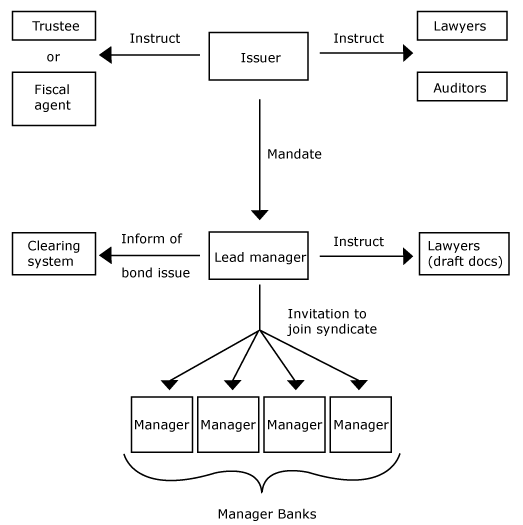
\includegraphics{C:/Users/shiva/Filen/MEGA/LegalPracticeCourse/bond-parties.png}

Attraction of euromarkets: speed of fund-raising. Can be 3 weeks for a
stand-alone bond. ICMA recommendations have developed a guideline
timetable of the issue process. Responsibility of lead manager and
solicitor to ensure this is followed..

\hypertarget{stages}{%
\subsection{Stages}\label{stages}}

\begin{enumerate}
\tightlist
\item
  Mandate
\item
  Due diligence
\item
  Documentation process begins
\item
  Marketing
\item
  Launch and syndication
\item
  Listing
\item
  Signing
\item
  Closing
\end{enumerate}

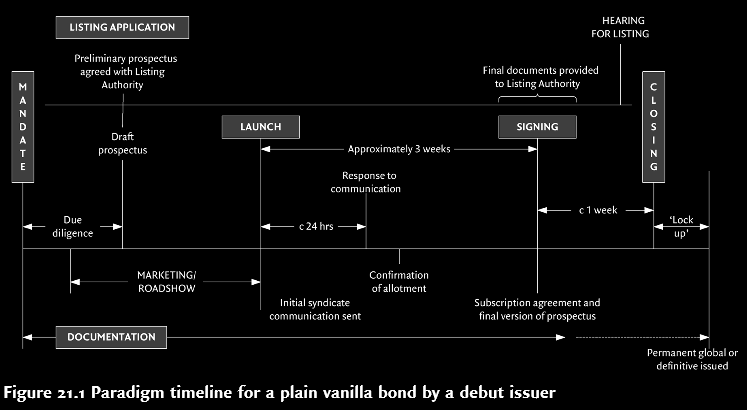
\includegraphics{C:/Users/shiva/Filen/MEGA/LegalPracticeCourse/bond-issue.png}

\hypertarget{mandate}{%
\subsection{Mandate}\label{mandate}}

= instructing an investment bank to lead-manage the issue.

Once appointed, the lead manager advises on the most appropriate
structure for an issue and the best market. Issuer and lead manager must
agree:

\begin{itemize}
\tightlist
\item
  Marketing strategy
\item
  Whether to list
\item
  Identities of fiscal agent/ trustee and paying agents
\item
  Fee structure
\end{itemize}

Recorded in mandate letter/ term sheet, drafted by the lead manager.

\hypertarget{due-diligence}{%
\subsection{Due Diligence}\label{due-diligence}}

Bond issues require due diligence in which the lead manager verifies
information needed for the issue. As a general rule, the due diligence
process for an issue of equity linked securities will be more `in depth'
than for a straight debt issue, since investors in the former may become
shareholders in the issuer (different risk).

The lead manager usually conducts the due diligence meeting by asking
detailed questions about the other parties to obtain sufficient
information to proceed with the issue/ prepare the prospectus.
Alternative: draft lots of questions.

Helps to provide material for the prospectus. Obtaining the comfort
letters in agreed form from the issuer's auditors is also part of the
due diligence process

\hypertarget{documentation}{%
\subsection{Documentation}\label{documentation}}

If the bond issue is to be listed, a draft of the prospectus or listing
particulars must be sent to the appropriate listing authority. The UKLA
usually requires a period of at least 10 working days in which to review
a prospectus prior to its intended publication (or 20 working days if
the issuer has not previously admitted securities to trading or made a
public offer).

\begin{itemize}
\tightlist
\item
  Prospectus.
\item
  Subscription agreement.
\item
  Agreement among managers.
\item
  Fiscal agency agreement and deed of covenant.*
\item
  Trust deed and paying agency agreement.*
\item
  Global note.
\item
  Legal opinion.
\item
  Signing and closing memorandum.
\end{itemize}

\hypertarget{marketing}{%
\subsection{Marketing}\label{marketing}}

Lead manager helps the issuer's directors in roadshows to potential
investors. Check roadshow material to ensure it complies with ss 21 and
25 of the FSMA 2000.

\begin{env-9f1ad080-32f6-4f2b-8995-b682d7bd2848}

Note

Sections 21--25 of the FSMA 2000 make it an offence for any person other
than an `authorised person' (ie, authorised to carry on regulated
activity under the FSMA 2000) to `in the course of business, communicate
an invitation or inducement to engage in investment activity' (or to
cause the same) in the UK, unless its contents have been approved by an
authorised person (or an exemption applies).

\end{env-9f1ad080-32f6-4f2b-8995-b682d7bd2848}

\hypertarget{launch-and-syndication}{%
\subsection{Launch and Syndication}\label{launch-and-syndication}}

Launch date confirmed by formal public announcement. Launch must await
completion of due diligence/ marketing. On launch, the issue is
announced to the market and the lead manager sends an initial syndicate
communication to financial institutions chosen to be invited into the
syndicate. Invitation shows the price of the bonds and fees/ commissions
to syndicate bank. Co-managers required to respond to the invitation
within 24 hours of receipt. Acceptance does not constitute a binding
contract to subscribe: that is the purpose of the subscription agreement
-- moral obligation.

The invitation telex usually includes the following:

\begin{itemize}
\tightlist
\item
  \textbf{Terms.} Proposed terms of the bond issue.
\item
  \textbf{Selling restrictions.} Any relevant selling restrictions that
  apply to the issue.
\item
  \textbf{Fees.} The fees of the managers.
\item
  \textbf{Agreement among managers.} Which version of the two
  industry-standard agreements among managers is to be used.
\end{itemize}

Once all the co-managers have responded, the lead manager will know the
level of interest in the issue, and can notify each co-manager of the
number of bonds it is expected to take at issue by way of a confirmation
of allotment. Once the confirmation of allotment has been sent, the
draft subscription agreement is sent to each co-manager.

\hypertarget{listing}{%
\subsection{Listing}\label{listing}}

A listed bond is one which is formally quoted, listed or capable of
being traded on a recognised stock exchange.

Reasons:

\begin{itemize}
\tightlist
\item
  To demonstrate that a bond has satisfied the requirements of the
  exchange - attaining listed status makes a bond more marketable.
\item
  Some entities are precluded from investing in securities which are not
  listed.
\item
  One specific advantage of obtaining a London listing of bonds is the
  `quoted bond exemption' from UK withholding tax. This exemption allows
  a UK issuer to pay gross interest on both bearer and registered bonds.
\end{itemize}

Disadvantages:

\begin{itemize}
\tightlist
\item
  Cost

  \begin{itemize}
  \tightlist
  \item
    Listing authorities charge a fee
  \item
    Lead manager fees and legal fees higher
  \end{itemize}
\item
  Timing

  \begin{itemize}
  \tightlist
  \item
    Longer timetable UKLA needs time to review documentation \& more DD
  \end{itemize}
\end{itemize}

\hypertarget{listing-requirements}{%
\subsubsection{Listing Requirements}\label{listing-requirements}}

See Listing Rule 2. The Stock Exchange reserves the right to impose any
special condition it considers appropriate in the interests of
protecting investors. These include:

\begin{itemize}
\tightlist
\item
  Status

  \begin{itemize}
  \tightlist
  \item
    Issuer duly incorporated and operating in conformity with
    constitution.
  \end{itemize}
\item
  Securities

  \begin{itemize}
  \tightlist
  \item
    Conditions:

    \begin{itemize}
    \tightlist
    \item
      Conform to law of issuer's place of incorporation, etc.
    \item
      Freely transferrable
    \item
      Expected aggregate market value of at least £200,000
    \item
      Entire class of a security must be listed
    \item
      Convertible securities must convert into securities themselves
      listed.
    \end{itemize}
  \end{itemize}
\end{itemize}

\hypertarget{application-procedure}{%
\subsubsection{Application Procedure}\label{application-procedure}}

LR 3, LR 17, PRR 3.

\hypertarget{clear-business-day-documents}{%
\paragraph{10 Clear Business Day
Documents}\label{clear-business-day-documents}}

Issuers (through their sponsor) must submit two copies of specified
documents to the UKLA at least 10 clear business days prior to their
intended publication (see PRR 3.1.6).

For a bond issue, these documents are:

\begin{itemize}
\tightlist
\item
  Requisite application form
\item
  Prospectus (annotated to indicate compliance)
\item
  2 letters (non-applicable letter and omission of information letter)
  explaining why some information does not appear).
\end{itemize}

\hypertarget{marked-up-documents}{%
\paragraph{Marked-up Documents}\label{marked-up-documents}}

Any 10-day documents which the UKLA amends (or which are altered after
submission to the UKLA) must be re-submitted with the changes marked up.

\hypertarget{hour-documents}{%
\paragraph{48-hour Documents}\label{hour-documents}}

Listing Rule 3.4.4 requires the following documents, in final form, to
be submitted at least two business days prior to the consideration of
the listing application:

\begin{enumerate}
\tightlist
\item
  a complete application for admission of the securities, and
\item
  either:

  \begin{enumerate}
  \tightlist
  \item
    the approved prospectus or listing particulars; or
  \item
    a copy of a prospectus approved by another Member State (under the
    `passporting' regime).
  \end{enumerate}
\end{enumerate}

\hypertarget{listing-charge}{%
\paragraph{Listing Charge}\label{listing-charge}}

On the day of consideration of the listing application, the issuer must
pay the appropriate listing fee (Listing Rule 3.2.2).

There are also continuing obligations.

\hypertarget{signing}{%
\subsection{Signing}\label{signing}}

Usually within 2 weeks of the issue being launched. Lead manager and
solicitors must be sure that aspects of the issue process have been
completed before signing.

Lead manager's solicitors should ensure:

\begin{itemize}
\tightlist
\item
  Prospectus is in agreed form
\item
  Other contractual documents completed
\item
  Resolutions necesssary to authorise issue executed
\item
  Common depository appointed.
\end{itemize}

\hypertarget{closing}{%
\subsection{Closing}\label{closing}}

Takes place \textasciitilde1 week after signing. Issuer receives funds
and bonds come into being. Lead manager's solicitors will produce an
agenda to ensure necessary matters completed.

\hypertarget{documentary-procedures}{%
\subsubsection{Documentary Procedures}\label{documentary-procedures}}

Lead manager's solicitor to complete before closing;

\begin{itemize}
\tightlist
\item
  Admission to listing
\item
  CPs to subscription agreement satisfied
\item
  Auditors' closing comfort letter and issuer's closing certificate
\item
  Legal opinions
\end{itemize}

By the end of completion, execute:

\begin{itemize}
\tightlist
\item
  Trust deed
\item
  Fiscal agency agreement/ paying agency agreement
\item
  Auditors' closing comfort letter
\item
  Legal opinions
\item
  Issuer's closing certificate
\item
  Payment instructions from lead manager
\item
  Temporary global note
\item
  Permanent global note, if any
\item
  Receipts between issuer and lead manager.
\end{itemize}

Temporary global note authenticated by the fiscal agent to give it legal
effect and delivered to the depository for safe-keeping.

After closing, any documents still to be lodged with UKLA must be sent
to the listing agent.

\hypertarget{payment-procedures}{%
\subsubsection{Payment Procedures}\label{payment-procedures}}

Closing mechanics/ payment against delivery procedures involved in most
transactions.

\hypertarget{prior-to-closing}{%
\paragraph{Prior to Closing}\label{prior-to-closing}}

The lead manager will have notified the clearing system of the names and
amounts of bonds to be allotted to the account of each syndicate member.
Each syndicate member will also give payment instructions to the
clearing system to the effect that its cash account is to be debited.

The instructions are phrased so that the debit will be made only if the
syndicate member is credited with the requisite number of bonds in its
securities account (payment against delivery).

The lead manager will also instruct the clearing system to debit its new
issues account with the total amount of the issue to be paid to the
account of the common depository.

\hypertarget{at-closing}{%
\paragraph{At Closing}\label{at-closing}}

The lead manager will authorise release of its payment instruction to
the depository to transfer the money (already placed with the
depository) representing the issue amount to the issuer. The depository
will transfer the money to the issuer's bank account upon receiving the
temporary global note.

The closing is now complete: the issuer has its funds and the depository
holds the temporary global note on behalf of the clearing system. The
clearing system will have credited the securities accounts of each
syndicate member.

\hypertarget{payment-against-delivery}{%
\subsubsection{Payment Against
Delivery}\label{payment-against-delivery}}

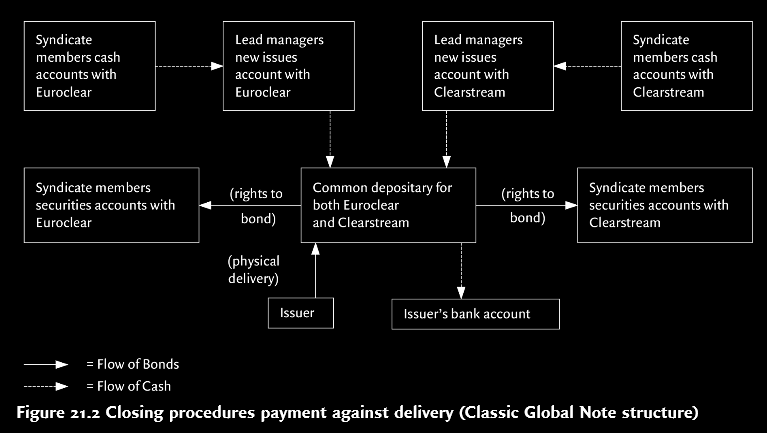
\includegraphics{C:/Users/shiva/Filen/MEGA/LegalPracticeCourse/bond-clearing.png}

\end{document}
